\documentclass[12pt]{article}
\usepackage[margin=0.1in]{geometry}
\usepackage[nomarkers,nofiglist,notablist]{endfloat}
\usepackage{xcolor}
\usepackage{framed}
\usepackage{enumitem}
\usepackage{adjustbox}
\usepackage{natbib}
\usepackage{chngpage}
\usepackage{mathtools,xparse}
\usepackage{graphics}
\usepackage{tikz}
\usepackage{tabu}
\usepackage{tikz-cd}
\colorlet{shadecolor}{orange!15}
% \definecolor{shadecolor}{rgb}{255,128,0}\
\usepackage{float}
\usepackage{fullpage} % Package to use full page
\usepackage{parskip} % Package to tweak paragraph skipping
\usepackage{amsmath}
\usepackage{amssymb}
\usepackage{hyperref}
\usepackage{pdflscape}
\usepackage{setspace}
\usepackage{graphicx} % Allows including images
\usepackage{booktabs} % Allows the use of \toprule, \midrule and \bottomrule in tables
\usepackage{longtable}
\usepackage{indentfirst}
\usetikzlibrary{arrows,shapes,positioning,shadows,trees}
\usepackage{array}
\usepackage{wrapfig}
\usepackage{multirow}
\usepackage{pdflscape}
\usepackage{threeparttable}
\usepackage{makecell}
\usepackage[normalem]{ulem}
\newcommand{\PreserveBackslash}[1]{\let\temp=\\#1\let\\=\temp}
\newcolumntype{L}[1]{>{\PreserveBackslash\raggedright}m{#1}}
\newcolumntype{R}[1]{>{\PreserveBackslash}p{#1}}
\newcolumntype{C}[1]{>{\PreserveBackslash\centering}m{#1}}
\newcommand{\Var}[1]{\text{Var}\left(#1\right)}
\newcommand{\mc}[3]{\multicolumn{#1}{#2}{#3}}

\tikzset{
  basic/.style  = {draw, text width=2cm, drop shadow, font=\sffamily, rectangle},
  root/.style   = {basic, rounded corners=2pt, thin, align=center,
                   fill=green!30},
  level 2/.style = {basic, rounded corners=6pt, thin,align=center, fill=green!60,
                   text width=8em},
  level 3/.style = {basic, thin, align=left, fill=pink!60, text width=6.5em}
}


\newcommand\independent{\protect\mathpalette{\protect\independenT}{\perp}}
\newcommand\gamij{\mathbf{\gamma_{ij}}}
\def\independenT#1#2{\mathrel{\rlap{$#1#2$}\mkern2mu{#1#2}}}
\newcommand\params{(p_M, p_{M\ell}, p_{U\ell})}
\newcommand\longparam{(L,n_1,n_2, p_M,p_{M\ell},p_{U\ell})}


%Allows multi-column tables 
% Macros for Scientific Word and Scientific WorkPlace 5.5 documents saved with the LaTeX filter.
% Copyright (C) 2005 Mackichan Software, Inc.

\typeout{TCILATEX Macros for Scientific Word and Scientific WorkPlace 5.5 <06 Oct 2005>.}
\typeout{NOTICE:  This macro file is NOT proprietary and may be 
freely copied and distributed.}
%
\makeatletter

%%%%%%%%%%%%%%%%%%%%%
% pdfTeX related.
\ifx\pdfoutput\relax\let\pdfoutput=\undefined\fi
\newcount\msipdfoutput
\ifx\pdfoutput\undefined
\else
 \ifcase\pdfoutput
 \else 
    \msipdfoutput=1
    \ifx\paperwidth\undefined
    \else
      \ifdim\paperheight=0pt\relax
      \else
        \pdfpageheight\paperheight
      \fi
      \ifdim\paperwidth=0pt\relax
      \else
        \pdfpagewidth\paperwidth
      \fi
    \fi
  \fi  
\fi

%%%%%%%%%%%%%%%%%%%%%
% FMTeXButton
% This is used for putting TeXButtons in the 
% frontmatter of a document. Add a line like
% \QTagDef{FMTeXButton}{101}{} to the filter 
% section of the cst being used. Also add a
% new section containing:
%     [f_101]
%     ALIAS=FMTexButton
%     TAG_TYPE=FIELD
%     TAG_LEADIN=TeX Button:
%
% It also works to put \defs in the preamble after 
% the \input tcilatex
\def\FMTeXButton#1{#1}
%
%%%%%%%%%%%%%%%%%%%%%%
% macros for time
\newcount\@hour\newcount\@minute\chardef\@x10\chardef\@xv60
\def\tcitime{
\def\@time{%
  \@minute\time\@hour\@minute\divide\@hour\@xv
  \ifnum\@hour<\@x 0\fi\the\@hour:%
  \multiply\@hour\@xv\advance\@minute-\@hour
  \ifnum\@minute<\@x 0\fi\the\@minute
  }}%

%%%%%%%%%%%%%%%%%%%%%%
% macro for hyperref and msihyperref
%\@ifundefined{hyperref}{\def\hyperref#1#2#3#4{#2\ref{#4}#3}}{}

\def\x@hyperref#1#2#3{%
   % Turn off various catcodes before reading parameter 4
   \catcode`\~ = 12
   \catcode`\$ = 12
   \catcode`\_ = 12
   \catcode`\# = 12
   \catcode`\& = 12
   \catcode`\% = 12
   \y@hyperref{#1}{#2}{#3}%
}

\def\y@hyperref#1#2#3#4{%
   #2\ref{#4}#3
   \catcode`\~ = 13
   \catcode`\$ = 3
   \catcode`\_ = 8
   \catcode`\# = 6
   \catcode`\& = 4
   \catcode`\% = 14
}

\@ifundefined{hyperref}{\let\hyperref\x@hyperref}{}
\@ifundefined{msihyperref}{\let\msihyperref\x@hyperref}{}




% macro for external program call
\@ifundefined{qExtProgCall}{\def\qExtProgCall#1#2#3#4#5#6{\relax}}{}
%%%%%%%%%%%%%%%%%%%%%%
%
% macros for graphics
%
\def\FILENAME#1{#1}%
%
\def\QCTOpt[#1]#2{%
  \def\QCTOptB{#1}
  \def\QCTOptA{#2}
}
\def\QCTNOpt#1{%
  \def\QCTOptA{#1}
  \let\QCTOptB\empty
}
\def\Qct{%
  \@ifnextchar[{%
    \QCTOpt}{\QCTNOpt}
}
\def\QCBOpt[#1]#2{%
  \def\QCBOptB{#1}%
  \def\QCBOptA{#2}%
}
\def\QCBNOpt#1{%
  \def\QCBOptA{#1}%
  \let\QCBOptB\empty
}
\def\Qcb{%
  \@ifnextchar[{%
    \QCBOpt}{\QCBNOpt}%
}
\def\PrepCapArgs{%
  \ifx\QCBOptA\empty
    \ifx\QCTOptA\empty
      {}%
    \else
      \ifx\QCTOptB\empty
        {\QCTOptA}%
      \else
        [\QCTOptB]{\QCTOptA}%
      \fi
    \fi
  \else
    \ifx\QCBOptA\empty
      {}%
    \else
      \ifx\QCBOptB\empty
        {\QCBOptA}%
      \else
        [\QCBOptB]{\QCBOptA}%
      \fi
    \fi
  \fi
}
\newcount\GRAPHICSTYPE
%\GRAPHICSTYPE 0 is for TurboTeX
%\GRAPHICSTYPE 1 is for DVIWindo (PostScript)
%%%(removed)%\GRAPHICSTYPE 2 is for psfig (PostScript)
\GRAPHICSTYPE=\z@
\def\GRAPHICSPS#1{%
 \ifcase\GRAPHICSTYPE%\GRAPHICSTYPE=0
   \special{ps: #1}%
 \or%\GRAPHICSTYPE=1
   \special{language "PS", include "#1"}%
%%%\or%\GRAPHICSTYPE=2
%%%  #1%
 \fi
}%
%
\def\GRAPHICSHP#1{\special{include #1}}%
%
% \graffile{ body }                                  %#1
%          { contentswidth (scalar)  }               %#2
%          { contentsheight (scalar) }               %#3
%          { vertical shift when in-line (scalar) }  %#4

\def\graffile#1#2#3#4{%
%%% \ifnum\GRAPHICSTYPE=\tw@
%%%  %Following if using psfig
%%%  \@ifundefined{psfig}{\input psfig.tex}{}%
%%%  \psfig{file=#1, height=#3, width=#2}%
%%% \else
  %Following for all others
  % JCS - added BOXTHEFRAME, see below
    \bgroup
	   \@inlabelfalse
       \leavevmode
       \@ifundefined{bbl@deactivate}{\def~{\string~}}{\activesoff}%
        \raise -#4 \BOXTHEFRAME{%
           \hbox to #2{\raise #3\hbox to #2{\null #1\hfil}}}%
    \egroup
}%
%
% A box for drafts
\def\draftbox#1#2#3#4{%
 \leavevmode\raise -#4 \hbox{%
  \frame{\rlap{\protect\tiny #1}\hbox to #2%
   {\vrule height#3 width\z@ depth\z@\hfil}%
  }%
 }%
}%
%
\newcount\@msidraft
\@msidraft=\z@
\let\nographics=\@msidraft
\newif\ifwasdraft
\wasdraftfalse

%  \GRAPHIC{ body }                                  %#1
%          { draft name }                            %#2
%          { contentswidth (scalar)  }               %#3
%          { contentsheight (scalar) }               %#4
%          { vertical shift when in-line (scalar) }  %#5
\def\GRAPHIC#1#2#3#4#5{%
   \ifnum\@msidraft=\@ne\draftbox{#2}{#3}{#4}{#5}%
   \else\graffile{#1}{#3}{#4}{#5}%
   \fi
}
%
\def\addtoLaTeXparams#1{%
    \edef\LaTeXparams{\LaTeXparams #1}}%
%
% JCS -  added a switch BoxFrame that can 
% be set by including X in the frame params.
% If set a box is drawn around the frame.

\newif\ifBoxFrame \BoxFramefalse
\newif\ifOverFrame \OverFramefalse
\newif\ifUnderFrame \UnderFramefalse

\def\BOXTHEFRAME#1{%
   \hbox{%
      \ifBoxFrame
         \frame{#1}%
      \else
         {#1}%
      \fi
   }%
}


\def\doFRAMEparams#1{\BoxFramefalse\OverFramefalse\UnderFramefalse\readFRAMEparams#1\end}%
\def\readFRAMEparams#1{%
 \ifx#1\end%
  \let\next=\relax
  \else
  \ifx#1i\dispkind=\z@\fi
  \ifx#1d\dispkind=\@ne\fi
  \ifx#1f\dispkind=\tw@\fi
  \ifx#1t\addtoLaTeXparams{t}\fi
  \ifx#1b\addtoLaTeXparams{b}\fi
  \ifx#1p\addtoLaTeXparams{p}\fi
  \ifx#1h\addtoLaTeXparams{h}\fi
  \ifx#1X\BoxFrametrue\fi
  \ifx#1O\OverFrametrue\fi
  \ifx#1U\UnderFrametrue\fi
  \ifx#1w
    \ifnum\@msidraft=1\wasdrafttrue\else\wasdraftfalse\fi
    \@msidraft=\@ne
  \fi
  \let\next=\readFRAMEparams
  \fi
 \next
 }%
%
%Macro for In-line graphics object
%   \IFRAME{ contentswidth (scalar)  }               %#1
%          { contentsheight (scalar) }               %#2
%          { vertical shift when in-line (scalar) }  %#3
%          { draft name }                            %#4
%          { body }                                  %#5
%          { caption}                                %#6


\def\IFRAME#1#2#3#4#5#6{%
      \bgroup
      \let\QCTOptA\empty
      \let\QCTOptB\empty
      \let\QCBOptA\empty
      \let\QCBOptB\empty
      #6%
      \parindent=0pt
      \leftskip=0pt
      \rightskip=0pt
      \setbox0=\hbox{\QCBOptA}%
      \@tempdima=#1\relax
      \ifOverFrame
          % Do this later
          \typeout{This is not implemented yet}%
          \show\HELP
      \else
         \ifdim\wd0>\@tempdima
            \advance\@tempdima by \@tempdima
            \ifdim\wd0 >\@tempdima
               \setbox1 =\vbox{%
                  \unskip\hbox to \@tempdima{\hfill\GRAPHIC{#5}{#4}{#1}{#2}{#3}\hfill}%
                  \unskip\hbox to \@tempdima{\parbox[b]{\@tempdima}{\QCBOptA}}%
               }%
               \wd1=\@tempdima
            \else
               \textwidth=\wd0
               \setbox1 =\vbox{%
                 \noindent\hbox to \wd0{\hfill\GRAPHIC{#5}{#4}{#1}{#2}{#3}\hfill}\\%
                 \noindent\hbox{\QCBOptA}%
               }%
               \wd1=\wd0
            \fi
         \else
            \ifdim\wd0>0pt
              \hsize=\@tempdima
              \setbox1=\vbox{%
                \unskip\GRAPHIC{#5}{#4}{#1}{#2}{0pt}%
                \break
                \unskip\hbox to \@tempdima{\hfill \QCBOptA\hfill}%
              }%
              \wd1=\@tempdima
           \else
              \hsize=\@tempdima
              \setbox1=\vbox{%
                \unskip\GRAPHIC{#5}{#4}{#1}{#2}{0pt}%
              }%
              \wd1=\@tempdima
           \fi
         \fi
         \@tempdimb=\ht1
         %\advance\@tempdimb by \dp1
         \advance\@tempdimb by -#2
         \advance\@tempdimb by #3
         \leavevmode
         \raise -\@tempdimb \hbox{\box1}%
      \fi
      \egroup%
}%
%
%Macro for Display graphics object
%   \DFRAME{ contentswidth (scalar)  }               %#1
%          { contentsheight (scalar) }               %#2
%          { draft label }                           %#3
%          { name }                                  %#4
%          { caption}                                %#5
\def\DFRAME#1#2#3#4#5{%
  \vspace\topsep
  \hfil\break
  \bgroup
     \leftskip\@flushglue
	 \rightskip\@flushglue
	 \parindent\z@
	 \parfillskip\z@skip
     \let\QCTOptA\empty
     \let\QCTOptB\empty
     \let\QCBOptA\empty
     \let\QCBOptB\empty
	 \vbox\bgroup
        \ifOverFrame 
           #5\QCTOptA\par
        \fi
        \GRAPHIC{#4}{#3}{#1}{#2}{\z@}%
        \ifUnderFrame 
           \break#5\QCBOptA
        \fi
	 \egroup
  \egroup
  \vspace\topsep
  \break
}%
%
%Macro for Floating graphic object
%   \FFRAME{ framedata f|i tbph x F|T }              %#1
%          { contentswidth (scalar)  }               %#2
%          { contentsheight (scalar) }               %#3
%          { caption }                               %#4
%          { label }                                 %#5
%          { draft name }                            %#6
%          { body }                                  %#7
\def\FFRAME#1#2#3#4#5#6#7{%
 %If float.sty loaded and float option is 'h', change to 'H'  (gp) 1998/09/05
  \@ifundefined{floatstyle}
    {%floatstyle undefined (and float.sty not present), no change
     \begin{figure}[#1]%
    }
    {%floatstyle DEFINED
	 \ifx#1h%Only the h parameter, change to H
      \begin{figure}[H]%
	 \else
      \begin{figure}[#1]%
	 \fi
	}
  \let\QCTOptA\empty
  \let\QCTOptB\empty
  \let\QCBOptA\empty
  \let\QCBOptB\empty
  \ifOverFrame
    #4
    \ifx\QCTOptA\empty
    \else
      \ifx\QCTOptB\empty
        \caption{\QCTOptA}%
      \else
        \caption[\QCTOptB]{\QCTOptA}%
      \fi
    \fi
    \ifUnderFrame\else
      \label{#5}%
    \fi
  \else
    \UnderFrametrue%
  \fi
  \begin{center}\GRAPHIC{#7}{#6}{#2}{#3}{\z@}\end{center}%
  \ifUnderFrame
    #4
    \ifx\QCBOptA\empty
      \caption{}%
    \else
      \ifx\QCBOptB\empty
        \caption{\QCBOptA}%
      \else
        \caption[\QCBOptB]{\QCBOptA}%
      \fi
    \fi
    \label{#5}%
  \fi
  \end{figure}%
 }%
%
%
%    \FRAME{ framedata f|i tbph x F|T }              %#1
%          { contentswidth (scalar)  }               %#2
%          { contentsheight (scalar) }               %#3
%          { vertical shift when in-line (scalar) }  %#4
%          { caption }                               %#5
%          { label }                                 %#6
%          { name }                                  %#7
%          { body }                                  %#8
%
%    framedata is a string which can contain the following
%    characters: idftbphxFT
%    Their meaning is as follows:
%             i, d or f : in-line, display, or floating
%             t,b,p,h   : LaTeX floating placement options
%             x         : fit contents box to contents
%             F or T    : Figure or Table. 
%                         Later this can expand
%                         to a more general float class.
%
%
\newcount\dispkind%

\def\makeactives{
  \catcode`\"=\active
  \catcode`\;=\active
  \catcode`\:=\active
  \catcode`\'=\active
  \catcode`\~=\active
}
\bgroup
   \makeactives
   \gdef\activesoff{%
      \def"{\string"}%
      \def;{\string;}%
      \def:{\string:}%
      \def'{\string'}%
      \def~{\string~}%
      %\bbl@deactivate{"}%
      %\bbl@deactivate{;}%
      %\bbl@deactivate{:}%
      %\bbl@deactivate{'}%
    }
\egroup

\def\FRAME#1#2#3#4#5#6#7#8{%
 \bgroup
 \ifnum\@msidraft=\@ne
   \wasdrafttrue
 \else
   \wasdraftfalse%
 \fi
 \def\LaTeXparams{}%
 \dispkind=\z@
 \def\LaTeXparams{}%
 \doFRAMEparams{#1}%
 \ifnum\dispkind=\z@\IFRAME{#2}{#3}{#4}{#7}{#8}{#5}\else
  \ifnum\dispkind=\@ne\DFRAME{#2}{#3}{#7}{#8}{#5}\else
   \ifnum\dispkind=\tw@
    \edef\@tempa{\noexpand\FFRAME{\LaTeXparams}}%
    \@tempa{#2}{#3}{#5}{#6}{#7}{#8}%
    \fi
   \fi
  \fi
  \ifwasdraft\@msidraft=1\else\@msidraft=0\fi{}%
  \egroup
 }%
%
% This macro added to let SW gobble a parameter that
% should not be passed on and expanded. 

\def\TEXUX#1{"texux"}

%
% Macros for text attributes:
%
\def\BF#1{{\bf {#1}}}%
\def\NEG#1{\leavevmode\hbox{\rlap{\thinspace/}{$#1$}}}%
%
%%%%%%%%%%%%%%%%%%%%%%%%%%%%%%%%%%%%%%%%%%%%%%%%%%%%%%%%%%%%%%%%%%%%%%%%
%
%
% macros for user - defined functions
\def\limfunc#1{\mathop{\rm #1}}%
\def\func#1{\mathop{\rm #1}\nolimits}%
% macro for unit names
\def\unit#1{\mathord{\thinspace\rm #1}}%

%
% miscellaneous 
\long\def\QQQ#1#2{%
     \long\expandafter\def\csname#1\endcsname{#2}}%
\@ifundefined{QTP}{\def\QTP#1{}}{}
\@ifundefined{QEXCLUDE}{\def\QEXCLUDE#1{}}{}
\@ifundefined{Qlb}{\def\Qlb#1{#1}}{}
\@ifundefined{Qlt}{\def\Qlt#1{#1}}{}
\def\QWE{}%
\long\def\QQA#1#2{}%
\def\QTR#1#2{{\csname#1\endcsname {#2}}}%
  %	Add aliases for the ulem package
  \let\QQQuline\uline
  \let\QQQsout\sout
  \let\QQQuuline\uuline
  \let\QQQuwave\uwave
  \let\QQQxout\xout
\long\def\TeXButton#1#2{#2}%
\long\def\QSubDoc#1#2{#2}%
\def\EXPAND#1[#2]#3{}%
\def\NOEXPAND#1[#2]#3{}%
\def\PROTECTED{}%
\def\LaTeXparent#1{}%
\def\ChildStyles#1{}%
\def\ChildDefaults#1{}%
\def\QTagDef#1#2#3{}%

% Constructs added with Scientific Notebook
\@ifundefined{correctchoice}{\def\correctchoice{\relax}}{}
\@ifundefined{HTML}{\def\HTML#1{\relax}}{}
\@ifundefined{TCIIcon}{\def\TCIIcon#1#2#3#4{\relax}}{}
\if@compatibility
  \typeout{Not defining UNICODE  U or CustomNote commands for LaTeX 2.09.}
\else
  \providecommand{\UNICODE}[2][]{\protect\rule{.1in}{.1in}}
  \providecommand{\U}[1]{\protect\rule{.1in}{.1in}}
  \providecommand{\CustomNote}[3][]{\marginpar{#3}}
\fi

\@ifundefined{lambdabar}{
      \def\lambdabar{\errmessage{You have used the lambdabar symbol. 
                      This is available for typesetting only in RevTeX styles.}}
   }{}

%
% Macros for style editor docs
\@ifundefined{StyleEditBeginDoc}{\def\StyleEditBeginDoc{\relax}}{}
%
% Macros for footnotes
\def\QQfnmark#1{\footnotemark}
\def\QQfntext#1#2{\addtocounter{footnote}{#1}\footnotetext{#2}}
%
% Macros for indexing.
%
\@ifundefined{TCIMAKEINDEX}{}{\makeindex}%
%
% Attempts to avoid problems with other styles
\@ifundefined{abstract}{%
 \def\abstract{%
  \if@twocolumn
   \section*{Abstract (Not appropriate in this style!)}%
   \else \small 
   \begin{center}{\bf Abstract\vspace{-.5em}\vspace{\z@}}\end{center}%
   \quotation 
   \fi
  }%
 }{%
 }%
\@ifundefined{endabstract}{\def\endabstract
  {\if@twocolumn\else\endquotation\fi}}{}%
\@ifundefined{maketitle}{\def\maketitle#1{}}{}%
\@ifundefined{affiliation}{\def\affiliation#1{}}{}%
\@ifundefined{proof}{\def\proof{\noindent{\bfseries Proof. }}}{}%
\@ifundefined{endproof}{\def\endproof{\mbox{\ \rule{.1in}{.1in}}}}{}%
\@ifundefined{newfield}{\def\newfield#1#2{}}{}%
\@ifundefined{chapter}{\def\chapter#1{\par(Chapter head:)#1\par }%
 \newcount\c@chapter}{}%
\@ifundefined{part}{\def\part#1{\par(Part head:)#1\par }}{}%
\@ifundefined{section}{\def\section#1{\par(Section head:)#1\par }}{}%
\@ifundefined{subsection}{\def\subsection#1%
 {\par(Subsection head:)#1\par }}{}%
\@ifundefined{subsubsection}{\def\subsubsection#1%
 {\par(Subsubsection head:)#1\par }}{}%
\@ifundefined{paragraph}{\def\paragraph#1%
 {\par(Subsubsubsection head:)#1\par }}{}%
\@ifundefined{subparagraph}{\def\subparagraph#1%
 {\par(Subsubsubsubsection head:)#1\par }}{}%
%%%%%%%%%%%%%%%%%%%%%%%%%%%%%%%%%%%%%%%%%%%%%%%%%%%%%%%%%%%%%%%%%%%%%%%%
% These symbols are not recognized by LaTeX
\@ifundefined{therefore}{\def\therefore{}}{}%
\@ifundefined{backepsilon}{\def\backepsilon{}}{}%
\@ifundefined{yen}{\def\yen{\hbox{\rm\rlap=Y}}}{}%
\@ifundefined{registered}{%
   \def\registered{\relax\ifmmode{}\r@gistered
                    \else$\m@th\r@gistered$\fi}%
 \def\r@gistered{^{\ooalign
  {\hfil\raise.07ex\hbox{$\scriptstyle\rm\text{R}$}\hfil\crcr
  \mathhexbox20D}}}}{}%
\@ifundefined{Eth}{\def\Eth{}}{}%
\@ifundefined{eth}{\def\eth{}}{}%
\@ifundefined{Thorn}{\def\Thorn{}}{}%
\@ifundefined{thorn}{\def\thorn{}}{}%
% A macro to allow any symbol that requires math to appear in text
\def\TEXTsymbol#1{\mbox{$#1$}}%
\@ifundefined{degree}{\def\degree{{}^{\circ}}}{}%
%
% macros for T3TeX files
\newdimen\theight
\@ifundefined{Column}{\def\Column{%
 \vadjust{\setbox\z@=\hbox{\scriptsize\quad\quad tcol}%
  \theight=\ht\z@\advance\theight by \dp\z@\advance\theight by \lineskip
  \kern -\theight \vbox to \theight{%
   \rightline{\rlap{\box\z@}}%
   \vss
   }%
  }%
 }}{}%
%
\@ifundefined{qed}{\def\qed{%
 \ifhmode\unskip\nobreak\fi\ifmmode\ifinner\else\hskip5\p@\fi\fi
 \hbox{\hskip5\p@\vrule width4\p@ height6\p@ depth1.5\p@\hskip\p@}%
 }}{}%
%
\@ifundefined{cents}{\def\cents{\hbox{\rm\rlap c/}}}{}%
\@ifundefined{tciLaplace}{\def\tciLaplace{\ensuremath{\mathcal{L}}}}{}%
\@ifundefined{tciFourier}{\def\tciFourier{\ensuremath{\mathcal{F}}}}{}%
\@ifundefined{textcurrency}{\def\textcurrency{\hbox{\rm\rlap xo}}}{}%
\@ifundefined{texteuro}{\def\texteuro{\hbox{\rm\rlap C=}}}{}%
\@ifundefined{euro}{\def\euro{\hbox{\rm\rlap C=}}}{}%
\@ifundefined{textfranc}{\def\textfranc{\hbox{\rm\rlap-F}}}{}%
\@ifundefined{textlira}{\def\textlira{\hbox{\rm\rlap L=}}}{}%
\@ifundefined{textpeseta}{\def\textpeseta{\hbox{\rm P\negthinspace s}}}{}%
%
\@ifundefined{miss}{\def\miss{\hbox{\vrule height2\p@ width 2\p@ depth\z@}}}{}%
%
\@ifundefined{vvert}{\def\vvert{\Vert}}{}%  %always translated to \left| or \right|
%
\@ifundefined{tcol}{\def\tcol#1{{\baselineskip=6\p@ \vcenter{#1}} \Column}}{}%
%
\@ifundefined{dB}{\def\dB{\hbox{{}}}}{}%        %dummy entry in column 
\@ifundefined{mB}{\def\mB#1{\hbox{$#1$}}}{}%   %column entry
\@ifundefined{nB}{\def\nB#1{\hbox{#1}}}{}%     %column entry (not math)
%
\@ifundefined{note}{\def\note{$^{\dag}}}{}%
%
\def\newfmtname{LaTeX2e}
% No longer load latexsym.  This is now handled by SWP, which uses amsfonts if necessary
%
\ifx\fmtname\newfmtname
  \DeclareOldFontCommand{\rm}{\normalfont\rmfamily}{\mathrm}
  \DeclareOldFontCommand{\sf}{\normalfont\sffamily}{\mathsf}
  \DeclareOldFontCommand{\tt}{\normalfont\ttfamily}{\mathtt}
  \DeclareOldFontCommand{\bf}{\normalfont\bfseries}{\mathbf}
  \DeclareOldFontCommand{\it}{\normalfont\itshape}{\mathit}
  \DeclareOldFontCommand{\sl}{\normalfont\slshape}{\@nomath\sl}
  \DeclareOldFontCommand{\sc}{\normalfont\scshape}{\@nomath\sc}
\fi

%
% Greek bold macros
% Redefine all of the math symbols 
% which might be bolded	 - there are 
% probably others to add to this list

\def\alpha{{\Greekmath 010B}}%
\def\beta{{\Greekmath 010C}}%
\def\gamma{{\Greekmath 010D}}%
\def\delta{{\Greekmath 010E}}%
\def\epsilon{{\Greekmath 010F}}%
\def\zeta{{\Greekmath 0110}}%
\def\eta{{\Greekmath 0111}}%
\def\theta{{\Greekmath 0112}}%
\def\iota{{\Greekmath 0113}}%
\def\kappa{{\Greekmath 0114}}%
\def\lambda{{\Greekmath 0115}}%
\def\mu{{\Greekmath 0116}}%
\def\nu{{\Greekmath 0117}}%
\def\xi{{\Greekmath 0118}}%
\def\pi{{\Greekmath 0119}}%
\def\rho{{\Greekmath 011A}}%
\def\sigma{{\Greekmath 011B}}%
\def\tau{{\Greekmath 011C}}%
\def\upsilon{{\Greekmath 011D}}%
\def\phi{{\Greekmath 011E}}%
\def\chi{{\Greekmath 011F}}%
\def\psi{{\Greekmath 0120}}%
\def\omega{{\Greekmath 0121}}%
\def\varepsilon{{\Greekmath 0122}}%
\def\vartheta{{\Greekmath 0123}}%
\def\varpi{{\Greekmath 0124}}%
\def\varrho{{\Greekmath 0125}}%
\def\varsigma{{\Greekmath 0126}}%
\def\varphi{{\Greekmath 0127}}%

\def\nabla{{\Greekmath 0272}}
\def\FindBoldGroup{%
   {\setbox0=\hbox{$\mathbf{x\global\edef\theboldgroup{\the\mathgroup}}$}}%
}

\def\Greekmath#1#2#3#4{%
    \if@compatibility
        \ifnum\mathgroup=\symbold
           \mathchoice{\mbox{\boldmath$\displaystyle\mathchar"#1#2#3#4$}}%
                      {\mbox{\boldmath$\textstyle\mathchar"#1#2#3#4$}}%
                      {\mbox{\boldmath$\scriptstyle\mathchar"#1#2#3#4$}}%
                      {\mbox{\boldmath$\scriptscriptstyle\mathchar"#1#2#3#4$}}%
        \else
           \mathchar"#1#2#3#4% 
        \fi 
    \else 
        \FindBoldGroup
        \ifnum\mathgroup=\theboldgroup % For 2e
           \mathchoice{\mbox{\boldmath$\displaystyle\mathchar"#1#2#3#4$}}%
                      {\mbox{\boldmath$\textstyle\mathchar"#1#2#3#4$}}%
                      {\mbox{\boldmath$\scriptstyle\mathchar"#1#2#3#4$}}%
                      {\mbox{\boldmath$\scriptscriptstyle\mathchar"#1#2#3#4$}}%
        \else
           \mathchar"#1#2#3#4% 
        \fi     	    
	  \fi}

\newif\ifGreekBold  \GreekBoldfalse
\let\SAVEPBF=\pbf
\def\pbf{\GreekBoldtrue\SAVEPBF}%
%

\@ifundefined{theorem}{\newtheorem{theorem}{Theorem}}{}
\@ifundefined{lemma}{\newtheorem{lemma}[theorem]{Lemma}}{}
\@ifundefined{corollary}{\newtheorem{corollary}[theorem]{Corollary}}{}
\@ifundefined{conjecture}{\newtheorem{conjecture}[theorem]{Conjecture}}{}
\@ifundefined{proposition}{\newtheorem{proposition}[theorem]{Proposition}}{}
\@ifundefined{axiom}{\newtheorem{axiom}{Axiom}}{}
\@ifundefined{remark}{\newtheorem{remark}{Remark}}{}
\@ifundefined{example}{\newtheorem{example}{Example}}{}
\@ifundefined{exercise}{\newtheorem{exercise}{Exercise}}{}
\@ifundefined{definition}{\newtheorem{definition}{Definition}}{}


\@ifundefined{mathletters}{%
  %\def\theequation{\arabic{equation}}
  \newcounter{equationnumber}  
  \def\mathletters{%
     \addtocounter{equation}{1}
     \edef\@currentlabel{\theequation}%
     \setcounter{equationnumber}{\c@equation}
     \setcounter{equation}{0}%
     \edef\theequation{\@currentlabel\noexpand\alph{equation}}%
  }
  \def\endmathletters{%
     \setcounter{equation}{\value{equationnumber}}%
  }
}{}

%Logos
\@ifundefined{BibTeX}{%
    \def\BibTeX{{\rm B\kern-.05em{\sc i\kern-.025em b}\kern-.08em
                 T\kern-.1667em\lower.7ex\hbox{E}\kern-.125emX}}}{}%
\@ifundefined{AmS}%
    {\def\AmS{{\protect\usefont{OMS}{cmsy}{m}{n}%
                A\kern-.1667em\lower.5ex\hbox{M}\kern-.125emS}}}{}%
\@ifundefined{AmSTeX}{\def\AmSTeX{\protect\AmS-\protect\TeX\@}}{}%
%

% This macro is a fix to eqnarray
\def\@@eqncr{\let\@tempa\relax
    \ifcase\@eqcnt \def\@tempa{& & &}\or \def\@tempa{& &}%
      \else \def\@tempa{&}\fi
     \@tempa
     \if@eqnsw
        \iftag@
           \@taggnum
        \else
           \@eqnnum\stepcounter{equation}%
        \fi
     \fi
     \global\tag@false
     \global\@eqnswtrue
     \global\@eqcnt\z@\cr}


\def\TCItag{\@ifnextchar*{\@TCItagstar}{\@TCItag}}
\def\@TCItag#1{%
    \global\tag@true
    \global\def\@taggnum{(#1)}%
    \global\def\@currentlabel{#1}}
\def\@TCItagstar*#1{%
    \global\tag@true
    \global\def\@taggnum{#1}%
    \global\def\@currentlabel{#1}}
%
%%%%%%%%%%%%%%%%%%%%%%%%%%%%%%%%%%%%%%%%%%%%%%%%%%%%%%%%%%%%%%%%%%%%%
%
\def\QATOP#1#2{{#1 \atop #2}}%
\def\QTATOP#1#2{{\textstyle {#1 \atop #2}}}%
\def\QDATOP#1#2{{\displaystyle {#1 \atop #2}}}%
\def\QABOVE#1#2#3{{#2 \above#1 #3}}%
\def\QTABOVE#1#2#3{{\textstyle {#2 \above#1 #3}}}%
\def\QDABOVE#1#2#3{{\displaystyle {#2 \above#1 #3}}}%
\def\QOVERD#1#2#3#4{{#3 \overwithdelims#1#2 #4}}%
\def\QTOVERD#1#2#3#4{{\textstyle {#3 \overwithdelims#1#2 #4}}}%
\def\QDOVERD#1#2#3#4{{\displaystyle {#3 \overwithdelims#1#2 #4}}}%
\def\QATOPD#1#2#3#4{{#3 \atopwithdelims#1#2 #4}}%
\def\QTATOPD#1#2#3#4{{\textstyle {#3 \atopwithdelims#1#2 #4}}}%
\def\QDATOPD#1#2#3#4{{\displaystyle {#3 \atopwithdelims#1#2 #4}}}%
\def\QABOVED#1#2#3#4#5{{#4 \abovewithdelims#1#2#3 #5}}%
\def\QTABOVED#1#2#3#4#5{{\textstyle 
   {#4 \abovewithdelims#1#2#3 #5}}}%
\def\QDABOVED#1#2#3#4#5{{\displaystyle 
   {#4 \abovewithdelims#1#2#3 #5}}}%
%
% Macros for text size operators:
%

\def\tint{\msi@int\textstyle\int}%
\def\tiint{\msi@int\textstyle\iint}%
\def\tiiint{\msi@int\textstyle\iiint}%
\def\tiiiint{\msi@int\textstyle\iiiint}%
\def\tidotsint{\msi@int\textstyle\idotsint}%
\def\toint{\msi@int\textstyle\oint}%


\def\tsum{\mathop{\textstyle \sum }}%
\def\tprod{\mathop{\textstyle \prod }}%
\def\tbigcap{\mathop{\textstyle \bigcap }}%
\def\tbigwedge{\mathop{\textstyle \bigwedge }}%
\def\tbigoplus{\mathop{\textstyle \bigoplus }}%
\def\tbigodot{\mathop{\textstyle \bigodot }}%
\def\tbigsqcup{\mathop{\textstyle \bigsqcup }}%
\def\tcoprod{\mathop{\textstyle \coprod }}%
\def\tbigcup{\mathop{\textstyle \bigcup }}%
\def\tbigvee{\mathop{\textstyle \bigvee }}%
\def\tbigotimes{\mathop{\textstyle \bigotimes }}%
\def\tbiguplus{\mathop{\textstyle \biguplus }}%
%
%
%Macros for display size operators:
%

\newtoks\temptoksa
\newtoks\temptoksb
\newtoks\temptoksc


\def\msi@int#1#2{%
 \def\@temp{{#1#2\the\temptoksc_{\the\temptoksa}^{\the\temptoksb}}}%   
 \futurelet\@nextcs
 \@int
}

\def\@int{%
   \ifx\@nextcs\limits
      \typeout{Found limits}%
      \temptoksc={\limits}%
	  \let\@next\@intgobble%
   \else\ifx\@nextcs\nolimits
      \typeout{Found nolimits}%
      \temptoksc={\nolimits}%
	  \let\@next\@intgobble%
   \else
      \typeout{Did not find limits or no limits}%
      \temptoksc={}%
      \let\@next\msi@limits%
   \fi\fi
   \@next   
}%

\def\@intgobble#1{%
   \typeout{arg is #1}%
   \msi@limits
}


\def\msi@limits{%
   \temptoksa={}%
   \temptoksb={}%
   \@ifnextchar_{\@limitsa}{\@limitsb}%
}

\def\@limitsa_#1{%
   \temptoksa={#1}%
   \@ifnextchar^{\@limitsc}{\@temp}%
}

\def\@limitsb{%
   \@ifnextchar^{\@limitsc}{\@temp}%
}

\def\@limitsc^#1{%
   \temptoksb={#1}%
   \@ifnextchar_{\@limitsd}{\@temp}%   
}

\def\@limitsd_#1{%
   \temptoksa={#1}%
   \@temp
}



\def\dint{\msi@int\displaystyle\int}%
\def\diint{\msi@int\displaystyle\iint}%
\def\diiint{\msi@int\displaystyle\iiint}%
\def\diiiint{\msi@int\displaystyle\iiiint}%
\def\didotsint{\msi@int\displaystyle\idotsint}%
\def\doint{\msi@int\displaystyle\oint}%

\def\dsum{\mathop{\displaystyle \sum }}%
\def\dprod{\mathop{\displaystyle \prod }}%
\def\dbigcap{\mathop{\displaystyle \bigcap }}%
\def\dbigwedge{\mathop{\displaystyle \bigwedge }}%
\def\dbigoplus{\mathop{\displaystyle \bigoplus }}%
\def\dbigodot{\mathop{\displaystyle \bigodot }}%
\def\dbigsqcup{\mathop{\displaystyle \bigsqcup }}%
\def\dcoprod{\mathop{\displaystyle \coprod }}%
\def\dbigcup{\mathop{\displaystyle \bigcup }}%
\def\dbigvee{\mathop{\displaystyle \bigvee }}%
\def\dbigotimes{\mathop{\displaystyle \bigotimes }}%
\def\dbiguplus{\mathop{\displaystyle \biguplus }}%

\if@compatibility\else
  % Always load amsmath in LaTeX2e mode
  \RequirePackage{amsmath}
\fi

\def\ExitTCILatex{\makeatother\endinput}

\bgroup
\ifx\ds@amstex\relax
   \message{amstex already loaded}\aftergroup\ExitTCILatex
\else
   \@ifpackageloaded{amsmath}%
      {\if@compatibility\message{amsmath already loaded}\fi\aftergroup\ExitTCILatex}
      {}
   \@ifpackageloaded{amstex}%
      {\if@compatibility\message{amstex already loaded}\fi\aftergroup\ExitTCILatex}
      {}
   \@ifpackageloaded{amsgen}%
      {\if@compatibility\message{amsgen already loaded}\fi\aftergroup\ExitTCILatex}
      {}
\fi
\egroup

%Exit if any of the AMS macros are already loaded.
%This is always the case for LaTeX2e mode.


%%%%%%%%%%%%%%%%%%%%%%%%%%%%%%%%%%%%%%%%%%%%%%%%%%%%%%%%%%%%%%%%%%%%%%%%%%
% NOTE: The rest of this file is read only if in LaTeX 2.09 compatibility
% mode. This section is used to define AMS-like constructs in the
% event they have not been defined.
%%%%%%%%%%%%%%%%%%%%%%%%%%%%%%%%%%%%%%%%%%%%%%%%%%%%%%%%%%%%%%%%%%%%%%%%%%
\typeout{TCILATEX defining AMS-like constructs in LaTeX 2.09 COMPATIBILITY MODE}
%%%%%%%%%%%%%%%%%%%%%%%%%%%%%%%%%%%%%%%%%%%%%%%%%%%%%%%%%%%%%%%%%%%%%%%%
%  Macros to define some AMS LaTeX constructs when 
%  AMS LaTeX has not been loaded
% 
% These macros are copied from the AMS-TeX package for doing
% multiple integrals.
%
\let\DOTSI\relax
\def\RIfM@{\relax\ifmmode}%
\def\FN@{\futurelet\next}%
\newcount\intno@
\def\iint{\DOTSI\intno@\tw@\FN@\ints@}%
\def\iiint{\DOTSI\intno@\thr@@\FN@\ints@}%
\def\iiiint{\DOTSI\intno@4 \FN@\ints@}%
\def\idotsint{\DOTSI\intno@\z@\FN@\ints@}%
\def\ints@{\findlimits@\ints@@}%
\newif\iflimtoken@
\newif\iflimits@
\def\findlimits@{\limtoken@true\ifx\next\limits\limits@true
 \else\ifx\next\nolimits\limits@false\else
 \limtoken@false\ifx\ilimits@\nolimits\limits@false\else
 \ifinner\limits@false\else\limits@true\fi\fi\fi\fi}%
\def\multint@{\int\ifnum\intno@=\z@\intdots@                          %1
 \else\intkern@\fi                                                    %2
 \ifnum\intno@>\tw@\int\intkern@\fi                                   %3
 \ifnum\intno@>\thr@@\int\intkern@\fi                                 %4
 \int}%                                                               %5
\def\multintlimits@{\intop\ifnum\intno@=\z@\intdots@\else\intkern@\fi
 \ifnum\intno@>\tw@\intop\intkern@\fi
 \ifnum\intno@>\thr@@\intop\intkern@\fi\intop}%
\def\intic@{%
    \mathchoice{\hskip.5em}{\hskip.4em}{\hskip.4em}{\hskip.4em}}%
\def\negintic@{\mathchoice
 {\hskip-.5em}{\hskip-.4em}{\hskip-.4em}{\hskip-.4em}}%
\def\ints@@{\iflimtoken@                                              %1
 \def\ints@@@{\iflimits@\negintic@
   \mathop{\intic@\multintlimits@}\limits                             %2
  \else\multint@\nolimits\fi                                          %3
  \eat@}%                                                             %4
 \else                                                                %5
 \def\ints@@@{\iflimits@\negintic@
  \mathop{\intic@\multintlimits@}\limits\else
  \multint@\nolimits\fi}\fi\ints@@@}%
\def\intkern@{\mathchoice{\!\!\!}{\!\!}{\!\!}{\!\!}}%
\def\plaincdots@{\mathinner{\cdotp\cdotp\cdotp}}%
\def\intdots@{\mathchoice{\plaincdots@}%
 {{\cdotp}\mkern1.5mu{\cdotp}\mkern1.5mu{\cdotp}}%
 {{\cdotp}\mkern1mu{\cdotp}\mkern1mu{\cdotp}}%
 {{\cdotp}\mkern1mu{\cdotp}\mkern1mu{\cdotp}}}%
%
%
%  These macros are for doing the AMS \text{} construct
%
\def\RIfM@{\relax\protect\ifmmode}
\def\text{\RIfM@\expandafter\text@\else\expandafter\mbox\fi}
\let\nfss@text\text
\def\text@#1{\mathchoice
   {\textdef@\displaystyle\f@size{#1}}%
   {\textdef@\textstyle\tf@size{\firstchoice@false #1}}%
   {\textdef@\textstyle\sf@size{\firstchoice@false #1}}%
   {\textdef@\textstyle \ssf@size{\firstchoice@false #1}}%
   \glb@settings}

\def\textdef@#1#2#3{\hbox{{%
                    \everymath{#1}%
                    \let\f@size#2\selectfont
                    #3}}}
\newif\iffirstchoice@
\firstchoice@true
%
%These are the AMS constructs for multiline limits.
%
\def\Let@{\relax\iffalse{\fi\let\\=\cr\iffalse}\fi}%
\def\vspace@{\def\vspace##1{\crcr\noalign{\vskip##1\relax}}}%
\def\multilimits@{\bgroup\vspace@\Let@
 \baselineskip\fontdimen10 \scriptfont\tw@
 \advance\baselineskip\fontdimen12 \scriptfont\tw@
 \lineskip\thr@@\fontdimen8 \scriptfont\thr@@
 \lineskiplimit\lineskip
 \vbox\bgroup\ialign\bgroup\hfil$\m@th\scriptstyle{##}$\hfil\crcr}%
\def\Sb{_\multilimits@}%
\def\endSb{\crcr\egroup\egroup\egroup}%
\def\Sp{^\multilimits@}%
\let\endSp\endSb
%
%
%These are AMS constructs for horizontal arrows
%
\newdimen\ex@
\ex@.2326ex
\def\rightarrowfill@#1{$#1\m@th\mathord-\mkern-6mu\cleaders
 \hbox{$#1\mkern-2mu\mathord-\mkern-2mu$}\hfill
 \mkern-6mu\mathord\rightarrow$}%
\def\leftarrowfill@#1{$#1\m@th\mathord\leftarrow\mkern-6mu\cleaders
 \hbox{$#1\mkern-2mu\mathord-\mkern-2mu$}\hfill\mkern-6mu\mathord-$}%
\def\leftrightarrowfill@#1{$#1\m@th\mathord\leftarrow
\mkern-6mu\cleaders
 \hbox{$#1\mkern-2mu\mathord-\mkern-2mu$}\hfill
 \mkern-6mu\mathord\rightarrow$}%
\def\overrightarrow{\mathpalette\overrightarrow@}%
\def\overrightarrow@#1#2{\vbox{\ialign{##\crcr\rightarrowfill@#1\crcr
 \noalign{\kern-\ex@\nointerlineskip}$\m@th\hfil#1#2\hfil$\crcr}}}%
\let\overarrow\overrightarrow
\def\overleftarrow{\mathpalette\overleftarrow@}%
\def\overleftarrow@#1#2{\vbox{\ialign{##\crcr\leftarrowfill@#1\crcr
 \noalign{\kern-\ex@\nointerlineskip}$\m@th\hfil#1#2\hfil$\crcr}}}%
\def\overleftrightarrow{\mathpalette\overleftrightarrow@}%
\def\overleftrightarrow@#1#2{\vbox{\ialign{##\crcr
   \leftrightarrowfill@#1\crcr
 \noalign{\kern-\ex@\nointerlineskip}$\m@th\hfil#1#2\hfil$\crcr}}}%
\def\underrightarrow{\mathpalette\underrightarrow@}%
\def\underrightarrow@#1#2{\vtop{\ialign{##\crcr$\m@th\hfil#1#2\hfil
  $\crcr\noalign{\nointerlineskip}\rightarrowfill@#1\crcr}}}%
\let\underarrow\underrightarrow
\def\underleftarrow{\mathpalette\underleftarrow@}%
\def\underleftarrow@#1#2{\vtop{\ialign{##\crcr$\m@th\hfil#1#2\hfil
  $\crcr\noalign{\nointerlineskip}\leftarrowfill@#1\crcr}}}%
\def\underleftrightarrow{\mathpalette\underleftrightarrow@}%
\def\underleftrightarrow@#1#2{\vtop{\ialign{##\crcr$\m@th
  \hfil#1#2\hfil$\crcr
 \noalign{\nointerlineskip}\leftrightarrowfill@#1\crcr}}}%
%%%%%%%%%%%%%%%%%%%%%

\def\qopnamewl@#1{\mathop{\operator@font#1}\nlimits@}
\let\nlimits@\displaylimits
\def\setboxz@h{\setbox\z@\hbox}


\def\varlim@#1#2{\mathop{\vtop{\ialign{##\crcr
 \hfil$#1\m@th\operator@font lim$\hfil\crcr
 \noalign{\nointerlineskip}#2#1\crcr
 \noalign{\nointerlineskip\kern-\ex@}\crcr}}}}

 \def\rightarrowfill@#1{\m@th\setboxz@h{$#1-$}\ht\z@\z@
  $#1\copy\z@\mkern-6mu\cleaders
  \hbox{$#1\mkern-2mu\box\z@\mkern-2mu$}\hfill
  \mkern-6mu\mathord\rightarrow$}
\def\leftarrowfill@#1{\m@th\setboxz@h{$#1-$}\ht\z@\z@
  $#1\mathord\leftarrow\mkern-6mu\cleaders
  \hbox{$#1\mkern-2mu\copy\z@\mkern-2mu$}\hfill
  \mkern-6mu\box\z@$}


\def\projlim{\qopnamewl@{proj\,lim}}
\def\injlim{\qopnamewl@{inj\,lim}}
\def\varinjlim{\mathpalette\varlim@\rightarrowfill@}
\def\varprojlim{\mathpalette\varlim@\leftarrowfill@}
\def\varliminf{\mathpalette\varliminf@{}}
\def\varliminf@#1{\mathop{\underline{\vrule\@depth.2\ex@\@width\z@
   \hbox{$#1\m@th\operator@font lim$}}}}
\def\varlimsup{\mathpalette\varlimsup@{}}
\def\varlimsup@#1{\mathop{\overline
  {\hbox{$#1\m@th\operator@font lim$}}}}

%
%Companion to stackrel
\def\stackunder#1#2{\mathrel{\mathop{#2}\limits_{#1}}}%
%
%
% These are AMS environments that will be defined to
% be verbatims if amstex has not actually been 
% loaded
%
%
\begingroup \catcode `|=0 \catcode `[= 1
\catcode`]=2 \catcode `\{=12 \catcode `\}=12
\catcode`\\=12 
|gdef|@alignverbatim#1\end{align}[#1|end[align]]
|gdef|@salignverbatim#1\end{align*}[#1|end[align*]]

|gdef|@alignatverbatim#1\end{alignat}[#1|end[alignat]]
|gdef|@salignatverbatim#1\end{alignat*}[#1|end[alignat*]]

|gdef|@xalignatverbatim#1\end{xalignat}[#1|end[xalignat]]
|gdef|@sxalignatverbatim#1\end{xalignat*}[#1|end[xalignat*]]

|gdef|@gatherverbatim#1\end{gather}[#1|end[gather]]
|gdef|@sgatherverbatim#1\end{gather*}[#1|end[gather*]]

|gdef|@gatherverbatim#1\end{gather}[#1|end[gather]]
|gdef|@sgatherverbatim#1\end{gather*}[#1|end[gather*]]


|gdef|@multilineverbatim#1\end{multiline}[#1|end[multiline]]
|gdef|@smultilineverbatim#1\end{multiline*}[#1|end[multiline*]]

|gdef|@arraxverbatim#1\end{arrax}[#1|end[arrax]]
|gdef|@sarraxverbatim#1\end{arrax*}[#1|end[arrax*]]

|gdef|@tabulaxverbatim#1\end{tabulax}[#1|end[tabulax]]
|gdef|@stabulaxverbatim#1\end{tabulax*}[#1|end[tabulax*]]


|endgroup
  

  
\def\align{\@verbatim \frenchspacing\@vobeyspaces \@alignverbatim
You are using the "align" environment in a style in which it is not defined.}
\let\endalign=\endtrivlist
 
\@namedef{align*}{\@verbatim\@salignverbatim
You are using the "align*" environment in a style in which it is not defined.}
\expandafter\let\csname endalign*\endcsname =\endtrivlist




\def\alignat{\@verbatim \frenchspacing\@vobeyspaces \@alignatverbatim
You are using the "alignat" environment in a style in which it is not defined.}
\let\endalignat=\endtrivlist
 
\@namedef{alignat*}{\@verbatim\@salignatverbatim
You are using the "alignat*" environment in a style in which it is not defined.}
\expandafter\let\csname endalignat*\endcsname =\endtrivlist




\def\xalignat{\@verbatim \frenchspacing\@vobeyspaces \@xalignatverbatim
You are using the "xalignat" environment in a style in which it is not defined.}
\let\endxalignat=\endtrivlist
 
\@namedef{xalignat*}{\@verbatim\@sxalignatverbatim
You are using the "xalignat*" environment in a style in which it is not defined.}
\expandafter\let\csname endxalignat*\endcsname =\endtrivlist




\def\gather{\@verbatim \frenchspacing\@vobeyspaces \@gatherverbatim
You are using the "gather" environment in a style in which it is not defined.}
\let\endgather=\endtrivlist
 
\@namedef{gather*}{\@verbatim\@sgatherverbatim
You are using the "gather*" environment in a style in which it is not defined.}
\expandafter\let\csname endgather*\endcsname =\endtrivlist


\def\multiline{\@verbatim \frenchspacing\@vobeyspaces \@multilineverbatim
You are using the "multiline" environment in a style in which it is not defined.}
\let\endmultiline=\endtrivlist
 
\@namedef{multiline*}{\@verbatim\@smultilineverbatim
You are using the "multiline*" environment in a style in which it is not defined.}
\expandafter\let\csname endmultiline*\endcsname =\endtrivlist


\def\arrax{\@verbatim \frenchspacing\@vobeyspaces \@arraxverbatim
You are using a type of "array" construct that is only allowed in AmS-LaTeX.}
\let\endarrax=\endtrivlist

\def\tabulax{\@verbatim \frenchspacing\@vobeyspaces \@tabulaxverbatim
You are using a type of "tabular" construct that is only allowed in AmS-LaTeX.}
\let\endtabulax=\endtrivlist

 
\@namedef{arrax*}{\@verbatim\@sarraxverbatim
You are using a type of "array*" construct that is only allowed in AmS-LaTeX.}
\expandafter\let\csname endarrax*\endcsname =\endtrivlist

\@namedef{tabulax*}{\@verbatim\@stabulaxverbatim
You are using a type of "tabular*" construct that is only allowed in AmS-LaTeX.}
\expandafter\let\csname endtabulax*\endcsname =\endtrivlist

% macro to simulate ams tag construct


% This macro is a fix to the equation environment
 \def\endequation{%
     \ifmmode\ifinner % FLEQN hack
      \iftag@
        \addtocounter{equation}{-1} % undo the increment made in the begin part
        $\hfil
           \displaywidth\linewidth\@taggnum\egroup \endtrivlist
        \global\tag@false
        \global\@ignoretrue   
      \else
        $\hfil
           \displaywidth\linewidth\@eqnnum\egroup \endtrivlist
        \global\tag@false
        \global\@ignoretrue 
      \fi
     \else   
      \iftag@
        \addtocounter{equation}{-1} % undo the increment made in the begin part
        \eqno \hbox{\@taggnum}
        \global\tag@false%
        $$\global\@ignoretrue
      \else
        \eqno \hbox{\@eqnnum}% $$ BRACE MATCHING HACK
        $$\global\@ignoretrue
      \fi
     \fi\fi
 } 

 \newif\iftag@ \tag@false
 
 \def\TCItag{\@ifnextchar*{\@TCItagstar}{\@TCItag}}
 \def\@TCItag#1{%
     \global\tag@true
     \global\def\@taggnum{(#1)}%
     \global\def\@currentlabel{#1}}
 \def\@TCItagstar*#1{%
     \global\tag@true
     \global\def\@taggnum{#1}%
     \global\def\@currentlabel{#1}}

  \@ifundefined{tag}{
     \def\tag{\@ifnextchar*{\@tagstar}{\@tag}}
     \def\@tag#1{%
         \global\tag@true
         \global\def\@taggnum{(#1)}}
     \def\@tagstar*#1{%
         \global\tag@true
         \global\def\@taggnum{#1}}
  }{}

\def\tfrac#1#2{{\textstyle {#1 \over #2}}}%
\def\dfrac#1#2{{\displaystyle {#1 \over #2}}}%
\def\binom#1#2{{#1 \choose #2}}%
\def\tbinom#1#2{{\textstyle {#1 \choose #2}}}%
\def\dbinom#1#2{{\displaystyle {#1 \choose #2}}}%

% Do not add anything to the end of this file.  
% The last section of the file is loaded only if 
% amstex has not been.
\makeatother
\endinput


\setlength{\topmargin}{-0.4in} 
\setlength{\textheight}{8.9in}
\setlength{\parindent}{2em}
% \setstretch{1.25}
\doublespacing
\title{\singlespacing Methods for analyzing linked data}
\author{Rachel Anderson\thanks{Mailing Address: Department of Economics, Julis Romo Rabinowitz Building,
Princeton, NJ 08544. Email: rachelsa@Princeton.edu.
This project received funding from the NIH (Grant 1 R01 HD077227-01). }}
\date{This Version: \today}

\begin{document}

\maketitle


\begin{abstract}
\singlespacing
\noindent This paper compares different methods for estimating parametric models with linked data, i.e. when $x$ and $y$ are observed in distinct datasets with imperfect identifiers.  This setup requires that the researcher must attempt to identify which observations in the $x$- and $y$-datafiles refer to the same individual, prior to performing inference about the joint or conditional distributions of $x$ and $y$.  At a minimum, random errors in the matching step introduce measurement error that must be accounted for in subsequent inference; however, additional concerns about sample selection arise when these errors are correlated with unobservables that affect $x$ or $y$.  \end{abstract}

% Using matched data requires estimation techniques that incorporate information from the matching process to improve efficiency and accurately reflect uncertainty. 

\newpage
\section{Introduction}

When analyzing multiple data sources with overlapping units, automated record linkage procedures offer the least cost solution for merging data.  These methods allow the researcher to specify a set of matching variables that are recorded across all of the datasets, and a decision rule for linking record pairs, in order to obtain a matched dataset in a matter of minutes.  When the files to be linked are large, the time saved relative to manual linking or automated linking with clerical review is immense. 

In the social sciences, interest in automated record linkage methods emerged in response to the increasing availability of administrative datasets, including recently digitized historical complete count population censuses.  Although these techniques originated in other fields -- primarily statistics, computer science, operations research, and epidemiology -- social scientists have developed their own linking methods in response to concerns about the accuracy and representativeness of data that are matched using imperfect identifiers.  

This new research agenda is driven by economic historians and historical demographers, who use data with identifiers that are prone to  typographical, duplication, enumeration, and digitization error.  Additionally, the identifiers may be misreported -- for example, ages may be rounded to integers ending with a 0 or 5 -- or repeated within a sample, as might happen if multiple Rachel Anderson's were born in the same year.  Historical record linkage procedures primarily differ according to how they address these issues of data quality. 

Examples of this literature include recent papers by \cite{abe2019} and \cite{bailey2017}, who compare the performance of popular historical record linkage methods to datasets matched by hand-linking or to simulated ``ground truth" datasets.  Although they implement different methods, both papers document a tradeoff between the false positive rate and the (true) match rate across procedures, and seem to agree that using more conservative algorithms leads to more representative data.  

Other contributions to this literature include papers by \cite{arp2018} and \cite{enamorado2019}, who demonstrate how to apply probabilistic record linkage methods from statistics to match historical and large-scale survey data.  These methods offer an advantage over the deterministic methods studied by \cite{abe2019} and \cite{bailey2017}, in that they can quantify the uncertainty about the matched data.  Furthermore, this extra information can be used to correct for bias introduced by false matches in the OLS estimator, using methods proposed by \cite{sw1993} and \cite{lahiri05}.

The ability to use probabilistic record linkage to correct for bias in the OLS estimator illustrates how the \textit{outputs} of different matching procedures determine which estimation methods are available for subsequent analysis.  Similarly, \cite{ahl2019} develop methods for consistently estimating GMM models using linked data that include multiple matches per observation.  Unfortunately, none of these estimation methods is acknowledged in the survey papers by \cite{abe2019} and \cite{bailey2017}; however, it seems natural that the choice of which matching procedure to use should be informed by which estimation methods are available. 

The goal of this paper is to build a bridge between the matching and estimation steps in the analysis of linked data.  I compare the performance  a comparison of different methods that incorporate different types of information, as well as extend the methods from \cite{ahl2019} to incorporate probabilities as may be outputted from a record linkage procedure.  

% good til here

% maybe add to intro Other methods for estimating with linked data are ad hoc or are not easily adapted to the setup in Section 2.  For example, \cite{bleakley2016} generated ``composite match" equal to the average of the linked observations.   \cite{nq2015} construct bounds on the parameter of interest using different configurations of matched data.   \cite{abe2012} use traditional estimation methods using only individuals who are uniquely matched, and then reweight on observables (not sure what this means?).   In statistics, authors have suggested using probabilistic record linkage and multiple imputation to correct for bias introduced by errors in the matching process \cite{sw1993, lahiri05, Goldstein2012}.   Multiple imputation is not useful here, as we do not consider missing data. The Lahiri methods require $N_x = N_y$ and so we are left with two methods.

By comparing the estimation methods, this gives suggestion to which record linkage procedure should be used (or, better yet, which outputs of the record linkage procedure are necessary for optimal estimation).  The main result is that unless probabilities can be estimated accurately, knowledge about them should not be incorporated in the estimation step.  

My preliminary results support the following suggestions for analyzing linked data: if you use deterministic matching, you should allow for multiple matches and use the estimator in \cite{ahl2019}.  If you use probabilistic record linkage, you should choose the match with the highest probability of being correct if it exceeds a certain threshold; otherwise you should use multiple matches because the estimated probabilities can be noisy, and can result in large weights on observations with small $\pi_{i\ell}$.  When it doubt, implement all methods and compare the results!

In order to illustrate the techniques studied in this paper, Section 2 introduces a numerical example that is used to demonstrate the matching and estimation techniques described in Sections 3 and 4.  Section 5 provides details about the implementation of the methods and data generating processes. �Section 6 contains the results, and Section 7 concludes.

%Each step of the record linkage process introduces the possibility that a true match is overlooked (Type II error), or that a false match is designated as correct (Type I error); and, generally, there is a tradeoff between reducing either one of the two \citep{abe2019, harron2018}.  Also representativeness is an issue. However, the impact of data pre-processing choices on estimation is still not well understood.  

%discussion can include where this may fail. 
%The example of \cite{aizer2016} illustrates how the choice of matching procedure determines which estimation methods are available.  Alternatively, the authors could have used probabilistic record linkage to estimate the probability that a given $(x_i, y_j)$ pair refers to a match, and incorporated this information into their estimation using the methods described in \cite{sw1993}.  

\section{Setup} 

In this section, I describe a simplified version of the estimation problem described in \cite{ahl2019}.  Whereas \cite{ahl2019} study how to incorporate multiple matches in a GMM framework, this paper focuses on estimating $\beta$ in the linear regression model, \begin{equation} y_i = x_i'\beta + \varepsilon_i, \ E[\varepsilon | x_i] = 0, \ E[\epsilon_i^2] = \sigma^2  \label{model} \end{equation}
where $x_i$ and $y_i$ are recorded in different datasets, and must be linked using auxiliary variables that are contained in both data sources.  

Formally, the data consist of observations $\{x_i, w_i\}_{i=1}^{N_x}$ in the $x$-datafile, and observations $\{y_j, w_j\}_{j=1}^{N_y}$ in the $y$-datafile.  I assume that $N_y\geq N_x$, and that every $x_i$ has a unique match in the $y$-datafile that satisfies the relationship in (\ref{model}), but the index $j$ that corresponds with the match is unknown.  Some $y_j$ may not correspond to any observation in the $x$ dataset, nor satisfy the relationship in (\ref{model}) for some unobserved $x_j$.  Hence, estimating the model in (\ref{model}) requires identifying which $(x_i,y_j)$ pairs refer to the same individuals by comparing $w_i$ and $w_j$ and designating matches according to some matching procedure. 
\addlinespace
\textbf{Example 1.}  To fix ideas, consider the work of \cite{aizer2016}, who seek to estimate the impact of providing cash transfers to single mothers on the life expectancy of their children.  The $x$-datafile consists of mothers' welfare program applications, where $x_i$ includes a binary variable equal to 1 if person $i$'s mother received a cash transfer, and other demographic variables.  The $y$-datafile is a universal database of death records, which includes $y_j$, person $j$'s age at death for all deaths reported to the Social Security Administration after 1965.  Both of the $x$- and $y$-datafiles also contain identifiers $w_i$ and $w_j$, which include first name, middle initial, last name, day, month, and year of birth, so that individuals with common names are not identified uniquely. 
\addlinespace
For the purposes of this paper, a matching procedure is defined as a set of rules used to construct a (potentially multi-valued) linking function, $\varphi: \{1,\dots, N_x\} \to \{1,\dots, N_y\} \cup \varnothing$, where $\varphi(i) = j$ if the $i$th observation in the $x$-datafile is matched to the $j$th observation in the $y$-datafile, and $\varphi(i) = \varnothing$ if $i$ is not assigned a match.  If $w_i$ and $w_j$ identify individuals uniquely and without error, then setting $\varphi(i) = j$ if and only if $w_i = w_j$, and $\varphi(i) = \varnothing$ otherwise, will correctly identify all true matches contained in the data.  In most applications, however, $w_i$ and $w_j$ cannot be used to unambiguously differentiate true matches, so that assigning $\varphi$ may include linking false matches or excluding true matches.  In this case, $\varphi$ may be constructed using estimates of $\pi_{ij}$, which denotes the probability that an $(i,j)$ pair refers to a match.  

\addlinespace
\textbf{Example 1 (cont'd).} \cite{aizer2016} construct $\varphi$ using a deterministic linking method that allows for errors in strings and dates of birth.  To account for changes in spelling and typographical errors, they convert all names into sounds using a phonetic algorithm, and measure the similarity between two individual's phonetically-spelled names using a string distance metric called SPEDIS.  They assign as matches all pairs of individuals whose birthdates fall within a predetermined range and whose SPEDIS score falls below a threshold.  Notably, their procedure does not enforce unique matches, so that some individuals are matched to multiple death records, and $\varphi$ is a correspondence. 
\addlinespace

Although I will discuss a few of the most popular methods used to construct $\varphi$ in later sections, this is not the focus of this paper.  Like \cite{ahl2019}, I take $\varphi$ and the matched dataset it produces as given.  The matched dataset can be written in the general form \begin{equation} \mathcal{D}_n \equiv \left(x_i, w_i, \{y_{i\ell}\}_{\ell=1}^{L_i}, \{\pi_{i\ell}\}_{\ell=1}^{L_i}\right)_{i=1}^N \label{data} \end{equation}
where $x_i$ is a vector of covariates for a single observation in the $x$-datafile, and $\{y_{i\ell}\}_{\ell=1}^{L_i}$ are the outcomes from the $y$-datafile to which it is linked based on the identifying variables $w_i$.  The variables $\{\pi_{i\ell}\}_{\ell=1}^{L_i}$ correspond to the conditional probability that a particular $y_{i\ell}$ refers to the correct match, so that $\sum_{\ell=1}^{L_i} \pi_{i\ell} = 1$.  If $\varphi$ was constructed without estimating $\pi_{i\ell}$, as in a deterministic matching procedure, I assume that $\pi_{i\ell} = \frac{1}{L_i}$.  

Additionally, I assume that (i) the true match $y_i$ is included among the possible matches $\{y_{i\ell}\}_{\ell=1}^{L_i}$ for all $i$, and that (ii) the observed $x_i$ and $\{y_{i\ell}\}_{\ell=1}^{L_i}$ are i.i.d. draws from their marginal distributions conditional on the identifying variables $w_i$.  Assumption (i) is necessary for identification, and Assumption (ii) is a selection on observables assumption, which requires that all individuals with the same identifying information are equally likely to be included in $\mathcal{D}_n$.  

Assumption (i) needs to be verified empirically; however the simulations in Section X suggest that it is reasonable when multiple matches are allowed.  Assumption (ii) requires thats all individuals with the same identifying information (such as name, age, Census block) have equal probability of appearing in the sample.  This assumption would be violated if, for example, higher income individuals have a greater probability of appearing in the sample (unless individuals are matched by income); but the OLS estimator using perfectly linked data would also be biased because of unobserved sample selection. 

\section{Estimation methods for linked data }

In this section, I review methods from \cite{sw1993} and \cite{ahl2019} (henceforth referred to as the SW and AHL estimators) for estimating regression models using matched data with the structure (\ref{data}), and establish conditions under which they are equivalent.   Although there are other methods for analyzing linked data, none is compatible with the setup described in Section 2.  For example, \cite{lahiri05} develop a version of the SW estimator based on the assumption that each observation in the $y$-datafile is generated by model in (\ref{model}), and that its corresponding value of $x$ appears in the $x$-datafile.  This differs from the problem considered in this paper, which allows for $N_y > N_x$, and assumes that the relationship in (\ref{model}) holds only for observations in the $x$-datafile. % Sentence about Goldstein.

\subsection{\cite{sw1993}}

Building upon the work \cite{NeterMaynes}, \cite{sw1993} study how to correct for bias introduced using incorrectly linked data in linear regression models.  Their methods assume that the data consist of observations $(x_i,z_i)_{i=1}^N$, so that each $x_i$ is linked with a single outcome $z_i$ that may or may not correspond to the true $y_i$.  Specifically, 
$$z_i = \begin{cases} y_i & \text{with probability $q_{ii}$} \\ y_j & \text{with probability $q_{ij}$ for $j\neq i,\ j = 1,\dots,N_y $} \end{cases}$$ 
and $\sum_{j=1}^{N_y} q_{ij} = 1, \ i=1,\dots, N$, where $N_y$ is the size of the $y$-datafile and $N$ is the size of the matched dataset.   Estimating (\ref{model}) using $z_i$ as the dependent variable yields the naive least squares estimator, 
\begin{equation} \hat{\beta}_N = (X'X)^{-1} X'z \label{naive} \end{equation}
which is biased, because $ E[z_i ] = E\left[q_{ii} y_i + \sum_{j\neq i} q_{ij} y_j\right] \neq E[y_i]$ if $q_{ii}\neq 1$ for some $i$.  Denoting
 $q_i = (q_{i1}, \dots, q_{iN_y})'$, \cite{sw1993} derive the bias of $\hat{\beta}_N $ conditional on the observed values of $y$,
\begin{equation} \text{bias} (\hat{\beta}_N | y) = E[(\hat{\beta}_N - \beta) | y ] = (X'X)^{-1} X'B \label{bias} \end{equation}
where $B = (B_1, \dots, B_n)'$ and $B_i = (q_{ii}-1)y_i + \sum_{j\neq i } q_{ij} y_j = q_i'y - y_i$, which is the difference between a weighted average of responses from all observations and the true response $y_i$.  

Observing (\ref{bias}), \cite{sw1993} propose estimating $\hat{B}$ using the first and second highest elements of $q_i$, and their corresponding values $y_j$ to compute 
\begin{equation} \hat{B}_i^{TR} = (q_{ij_1} - 1) y_{ij_1} + q_{ij_2} y_{ij_2} \label{bHat} \end{equation}
for each $i$, and then using it to correct for the bias in $\hat{\beta}_N$ as follows,
\begin{equation} \hat{\beta}_{SW} = \hat{\beta}_N - (X'X)^{-1} X' \hat{B}^{TR} \label{sw}\end{equation}
In principle, $\hat{B}^{TR}$ can incorporate any number of elements of $q_i$, however \cite{sw1993} show that if $q_{ij1}$ is sufficiently high for all $i$, then the truncation with two links results in a very small bias.  
 
The SW estimator has two important caveats.  The first is that it requires that the $y$ value associated with the largest element in $q_i$ corresponds with the true outcome $y_i$, so that errors in $z_i$ result from random assignment rules or requiring that no two values $x_i$ and $x_j$ are linked to the same value of $y$.  The second is that constructing $\hat{\beta}_{SW}$ requires knowledge of $q_{i}$ and the corresponding elements of $y$, and so it cannot be applied to data linked with deterministic methods.  Even if estimates of $q_{ij}$ are available, $\hat{\beta}_{SW}$ will be biased if the estimates $\widehat{q_{ij}}$ are correlated with $x$ or $y$, which occurs if $x$ or $y$ is correlated with errors in the matching variables.  This assumption is different from Assumption (ii) in Section 2, and often fails in economic application, such as in \cite{nq2015}, where $y$ measures whether a person's recorded ethnicity changes between Census years, and changes in first and last name (the matching variables) are strongly correlated with $y$.  

\subsection{\cite{ahl2019}}

Unlike the SW estimator, the estimator proposed in \cite{ahl2019} is unbiased under Assumptions (i) and (ii) from Section 2, and does not require estimates of $q_{ij}$.  Recall that the assumptions are that (i) the true match of $x_i$ is included among the matches $\{y_{i\ell}\}_{\ell=1}^{L_i}$ for all $i$, and (ii) $x_i$ and $y_i$ are random samples conditional on the matching variables.  Assumption (ii) allows $x$ and $y$ to be correlated with errors in matching, so long as that dependence is fully captured by $w$; hence the AHL estimator would be valid in the \cite{nq2015} example if ethnicity is included among the matching variables.  

The goal of \cite{ahl2019} is to estimate $\theta_0$ that satisfies the model
\begin{equation}
E_0\left[ m\left( y_{i},x_{i};\theta _{0}\right) \right] =0
\label{Moment}
\end{equation}%
where $y_{i}$ and $x_{i}$ are vectors or scalars of data for an individual $i$, the function $m(\cdot)$ is known, and the expectation is taken with respect to the joint distribution $f_0(y,x)$.  The data consist of observations $\left(x_i, w_i, \{y_{i\ell}\}_{\ell=1}^{L_i}\right)_{i=1}^N$, where the $x_i$ and $y_{i\ell}$ are recorded in distinct datasets and matched according to the identifier $w_i$.  They assume $L_i > 1$ for some $i$, so that the identity of the outcome that generates the relationship in (\ref{Moment}) is unknown.  

Under assumptions (i) and (ii) in Section 2, (\ref{Moment}) can be rewritten,
\begin{gather*}
E_0[m(y_i, x_i; \theta)] = E\left[\sum_{\ell=1}^{L_i} m(y_{i\ell}, x_i; \theta)\right] - E\left[(L_i -1)g(w_i, L_i; x_i; \theta)\right] \\ 
g(w_i, L_i, x_i; \theta) = E\left[m(y_i, x_i; \theta) |\ w_i, L_i \right] 
\end{gather*}
so if $g$ is known or can be estimated consistently, a sample version of (\ref{Moment}) can be constructed as follows,
\begin{equation}
\overline{m}_n(\theta, \hat{g}) = \frac{1}{N}\sum_{i=1}^N \sum_{\ell=1}^{L_i} m(y_{i\ell}, x_i ;\theta) - \frac{1}{N}\sum_{i=1}^N (L_i-1) \hat{g}(w_i, L_i, x_i; \theta) 
\label{ahl_moment}
\end{equation}
which is in general a two-step procedure, where $\hat{g}$ is estimated using nonparametric methods such as $k$-Nearest Neighbors or local polynomial regression in the first step.  The GMM estimator applied to (\ref{ahl_moment}) is consistent and asymptotically normal under the regularity conditions described in \cite{ahl2019}. 

For the linear regression model in (\ref{model}), the AHL estimator can be computed by applying OLS to the transformed regression model,
\begin{equation} 
\sum_{\ell=1}^{L_i} y_{i\ell} - (L_i - 1)\hat{g}(w_i, L_i) = x_i'\beta + u_i  \label{ahl} \end{equation}
where $\hat{g}(w_i,L_i)$ is a (possibly nonparametric) estimator of $E[y_{i\ell} | w_i, L_i ]$, $u_i = \varepsilon_i + \sum_{\ell=1}^{L_i}\nu_{i\ell}$, and $\nu_{i\ell} = y_{i\ell} - \hat{g}(w_i, L_i)$.   If, additionally, $E[\varepsilon_i^2 | x_i, w_i, L_i] = \sigma_{\varepsilon}^2$ and $E[\nu_{i\ell}^2 | x_i, w_i, L_i] = \sigma_{\nu}^2$ then the efficient estimator is weighted least squares,
\begin{equation}
\hat{\beta}^{WLS} = \left(\sum_{i=1}^N \frac{x_ix_i'}{\sigma(X_i)}\right)^{-1}\left(\sum_{i=1}^N \frac{x_i}{\sigma(X_i)}\left(\sum_{\ell=1}^{L_i} y_{i\ell} - (L_i - 1) g(w_i, L_i)\right)\right) \label{wls}
\end{equation}
where $\sigma(X_i) = \sigma_{\varepsilon}^2 + (L_i - 1)\sigma_{\nu}^2$.   

Unfortunately, the performance of the AHL estimator depends on the accuracy of $\hat{g}(w_i, L_i)$, which is a function of a potentially high-dimensional vector $w_i$ that may contain string or categorical variables.  However, if consider adding an assumption (iii) that $E[m(y_i, x_i; \theta) | L_i = \ell] = E_0[m(y_i, x_i; \theta)]$, then 
\begin{equation}
E_0[m(y_i, x_i; \theta)] = E\left[\sum_{\ell=1}^{L_i} m(y_{i\ell}, x_i; \theta) \Bigg|\ L_i = 2 \right]  - E\left[ \sum_{\ell=1}^{L_i} m(y_{i\ell}, x_i; \theta) \Bigg|\ L_i = 3\right] \label{new_ahl} \end{equation}
and
\begin{equation}
E_0[m(y_i, x_i; \theta)] = E[m(y_{i\ell}, x_i; \theta) | L_i =1]  \label{obs}
\end{equation}
So that we apply GMM to (\ref{new_ahl}) and (\ref{obs}) as the new moment conditions.  Applying this to the linear regression model (\ref{model}), yields the following moment conditions,
\begin{gather}
\begin{bmatrix} \frac{2}{N_{L_ 2}} \sum_{i=1}^{N_{L_2}} (y_{i1} + y_{i2} - x_i'\beta)x_i  - \frac{1}{N_{L_3}} \sum_{i=1}^{N_{L_3}} (y_{i1} + y_{i2} + y_{i3} - x_i'\beta)x_i   \\
\frac{1}{N_{L_1}}\sum_{i=1}^{N_{L_1}} (y_i - x_i'\beta)x_i \end{bmatrix} = 0 
\end{gather}
where $N_{L_{\ell}}$ is the number of observations matched to $\ell$ observations.  In practice, the precision of the estimator depends on the number of observations that are linked to two and three outcomes, however the estimator based on these moments should be asymptotically consistent.  % think about doing a proof

\subsection{Comparing $\hat{\beta}_{SW}$ and $\hat{\beta}_{AHL}$}
There is a natural parallel between $\hat{\beta}_{SW}$ and $\hat{\beta}_{AHL}$ when we consider data of the form in (\ref{data}), and we assume that $L_i$ is the number of links whose $q_{ij}$ exceed a threshold $\bar{q}$, and that the conditional probabilities $\pi_{i\ell} = \frac{q_{i\ell}}{\sum_{\ell=1}^{L_{i}} q_{i\ell}}$.  Let also $y_{i\ell^*}$ refer to the element of $\{y_{i\ell}\}_{\ell=1}^{L_i}$ that is associated with the highest value of $\{\pi_{i\ell}\}_{\ell=1}^{L_i}$.  Then, we can write $\hat{\beta}_{SW}$ as the OLS estimator for the model
\begin{equation}
z_i - \hat{B}_i = x_i'\beta + \varepsilon_i 
\label{transformed}
\end{equation}
with $\hat{B}_i = \sum_{\ell =1}^{L_i} \pi_{i\ell} y_{i\ell} - y_{i\ell^*}$.  Note that the \cite{sw1993} method assumes that the $y_{i\ell}$ with the highest value of $\pi_{i\ell}$ is the true match.\footnote{There are reasons that $z_i \neq y_{i\ell^*}$.  This happens, for example, if $z_i$ is assigned at random according to the probabilities $\pi_{i\ell}$ or if a one-to-one matching is enforced such that no single $y$ is assigned to two distinct values of $x$}

The AHL estimator can be written in the form (\ref{transformed}) with 
\begin{equation}
\hat{B}_i = z_i - \sum_{\ell=1}^{L_i} y_{i\ell} + (L_i -1) \hat{g}(w_i, L_i) \end{equation} 
so that $\hat{\beta}^{AHL}$ and $\hat{\beta}^{SW}$ differ only in their choice of $B_i$.  Alternatively, $\hat{\beta}_{SW}$ can be written in the form of $\hat{\beta}_{AHL}$, as in equation (\ref{ahl}), by setting 
\begin{equation} \hat{g}(w_i, L_i) = \frac{1}{L_i -1 }\left( \sum_{\ell \neq \ell^*} y_{i\ell} + y_{i\ell^*} \right) \label{ahl_sw} \end{equation}
Since $\hat{g}(\cdot)$ as written in (\ref{ahl_sw}) ignores information about $w_i$, and assumes that $y_{i\ell^*}$ is the correct match, the AHL estimator may perform better if $y_{i\ell^*}$ is not the true match, informative $\pi_{i\ell}$ are not available, or $w_i$ contains information about the conditional mean of the $y_{i\ell}$ drawn from the incorrect distribution.   However, if reliable estimates of $\pi_{i\ell}$ is available, it may be possible to improve the AHL estimator by incorporating this information.  I explore this possibility in the next section. 

\section{Incorporating probabilities in the AHL estimator} 

I begin by considering a simplified version of the AHL (2019) problem, based on the observation that 
$$ E[m(y_{i\ell}, x_i; \theta)] =  \begin{cases} 0 & \text{if } y_{i\ell} = y_i \\
g(w_i, L_i, x_i; \theta) & \text{if } y_{i\ell} \neq y_i
\end{cases} $$
If $\hat{g}$ can be estimated consistently, or $g(\cdot)$ is a constant function, this problem can be reduced to estimating the mean using observations $\{X_{i\ell}\}_{\ell=1}^{L_i}$, where each $X_{i\ell}$ is drawn from the correct distribution with probability $\pi_{i\ell}$ and drawn from the incorrect distribution with probability $(1-\pi_{i\ell})$.  Under Assumption (i), exactly one of the $X_{i\ell}$ is drawn from the correct distribution, so that $\sum_{\ell=1}^{L_i} X_{i\ell} = \mu + (L_i -1) \kappa$, where $\mu =0$ in the above example, and $\kappa = g(\cdot)$. 

\subsection{Estimating the mean}

Consider the problem of estimating the mean of a random variable $X \sim F_X(\mu; \sigma^2)$ using two observations $X_{1}$ and $X_{2}$.  With probability $\pi$, $X_1$ is drawn from the true distribution $F_X$ and $X_2$ is noise drawn from the distribution $F_Y(\kappa, \omega^2)$.  With probability $1-\pi$, $X_2$ is drawn from the correct distribution and $X_1$ is noise.  Under this specification, exactly one of $X_1$ or $X_2$ is drawn from the distribution of interest at all times.  

Observe that if $\pi$ is known, we can construct an unbiased estimator using only $X_1$,
\begin{equation}
\hat{\mu}_1 = \frac{X_1}{\pi} - \frac{1-\pi}{\pi} \kappa 
\label{mu1}
\end{equation} 
and, similarly, we can construct an unbiased estimator using only $X_2$,
\begin{equation}\hat{\mu_2} = \frac{X_2}{1-\pi} - \frac{\pi}{1-\pi} \kappa \label{mu2} \end{equation} 
Any unbiased linear estimator $\hat{\mu}$ that uses both $X_1$ and $X_2$ can be written as a combination of $\hat{\mu}_1$ and $\hat{\mu}_2$ (see Lemma 1 in the Appendix for a proof), so finding the minimum variance, unbiased linear estimator $\hat{\mu}$ requires minimizing 
$$\min_d\  \Var{d \hat{\mu}_1 + (1-d) \hat{\mu}_2}$$
which is solved by \begin{equation} d^*= \frac{\Var{\hat{\mu}_2} - \text{Cov}(\hat{\mu}_1, \hat{\mu}_2)}{\Var{\hat{\mu}_1} + \Var{\hat{\mu}_2} - 2 \text{Cov}(\hat{\mu}_1, \hat{\mu}_2)} \label{dOpt}\end{equation}
where
\begin{align} \Var{\hat{\mu}_1} &=  \frac{\text{Var}(X_1)}{\pi^2} = \frac{1}{\pi^2}\left(\pi \sigma^2 + (1-\pi) \omega^2 + \pi(1-\pi)(\mu-\kappa)^2\right) \label{vmu1}\\
\Var{\hat{\mu}_2} &= \frac{\Var{X_2}}{(1-\pi)^2} = \frac{1}{(1-\pi)^2}\left((1-\pi)\sigma^2 + \pi \omega^2 + \pi(1-\pi)(\mu-\kappa)^2\right)\label{vmu2} \\
\text{Cov}(\hat{\mu}_1, \hat{\mu}_2) &= \frac{\text{Cov}(X_1,X_2)}{\pi(1-\pi)} = \frac{1}{\pi(1-\pi)}\left((1-\pi^2 - (1-\pi)^2)\mu\kappa - \pi(1-\pi)(\mu^2 + \kappa^2)\right) \label{cov}
\end{align} 
Derivations of these formulas are in the appendix.

Thus, the minimum variance unbiased estimator is 
\begin{equation} \hat{\mu}^* \equiv \hat{\mu}(d^*) = d^* \hat{\mu}_1 + (1-d^*) \hat{\mu}_2 \label{muOpt}
\end{equation}
where $d^*$ is defined as in (\ref{dOpt}).  Note that $d^*$ is strictly increasing in $\pi$, but at a rate that depends on $\sigma^2, \omega^2, \mu,$ and $\kappa$.  Intuitively, this means that the optimal estimator $\hat{\mu}^*$ puts more weight on the observation that is most likely to be correct. 

Figure \ref{dStar} plots the optimal $d^*$ for $\pi\in[0,0.5]$, since the solution is symmetric in $\pi$ when $L=2$. When $\pi=0.5$, $\Var{\hat{\mu}_1}=\Var{\hat{\mu}_2}$ so that $d^*=0.5$, regardless of the other parameter values.  When the variance of both the correct and incorrect distributions are the same (i.e., $\sigma^2 = \omega^2$), then $\Var{X_1}=\Var{X_2}$, and differences in $d^*$ reflect only changes in $\pi$.   When $\sigma^2 \neq \omega^2$, the optimal $d^*$ puts additional weight (relative to the equal variance case) on the estimator based on the $X_i$ that is more likely to come from the lower variance distribution.  The curve with $\sigma^2 = 1$ and $\omega^2 = 10$ is the extreme version of this scenario, and represents what may happen if $\kappa$ is estimated imprecisely.  The resulting $d^*$ assigns very low weight to the observation that is more likely drawn from the incorrect distribution.  

\begin{figure}[htbp]
\begin{center}
\caption{Optimal $d^*$ as a function of $\pi$ and $\sigma^2, \omega^2, \mu, \kappa$}
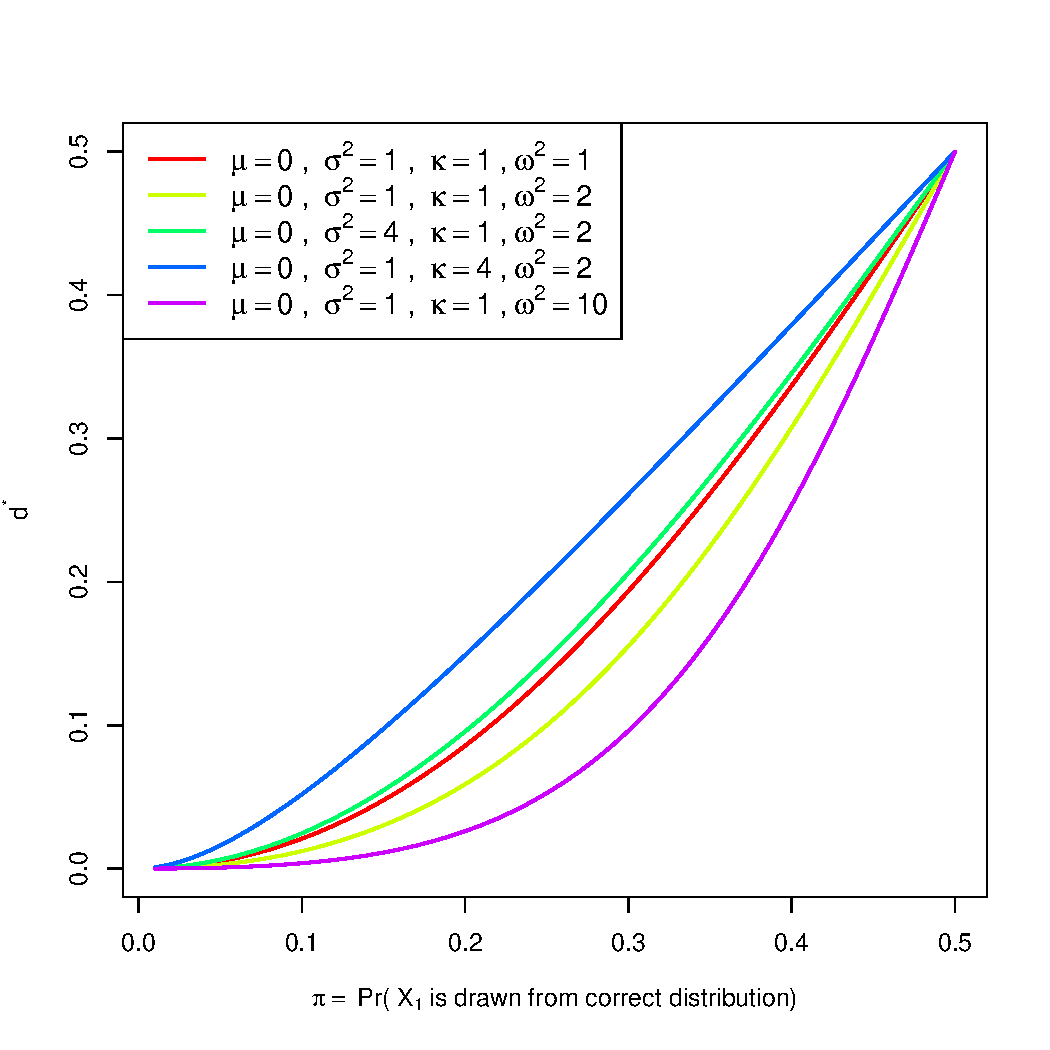
\includegraphics[width=0.8\textwidth]{./Figures/dStar.pdf}
\label{dStar}
\end{center}
\end{figure}

More generally, the estimator $\hat{\mu}^*$ can be computed for a sample of observations $(X_{i1}, X_{i2})_{i=1}^N$, where $X_{i1}$ is drawn from $F_X$ with probability $\pi_i$, and $X_{i2}$ is drawn from $F_X$ with probability $1-\pi_i$.  In this case, $d^*$ is calculated according to (\ref{dOpt}) using,
\begin{align*} \hat{\mu}_1 &= \sum_{i=1}^N \frac{X_{i1}}{\pi_i} - \frac{1-\pi_i}{\pi_i}\kappa 
& \Var{\hat{\mu}_1} &=  \frac{1}{N^2}\sum_{i=1}^N \frac{g(\pi_i; \theta)}{\pi_i^2} \\
 \hat{\mu}_2 &= \sum_{i=1}^N \frac{X_{i2}}{1-\pi_i} - \frac{\pi_i}{1-\pi_i}\kappa \ &\Var{\hat{\mu}_2} &= \frac{1}{N^2} \sum_{i=1}^N \frac{g(1-\pi_i; \theta)}{(1-\pi_i)^2} \end{align*}
$$\text{Cov}(\hat{\mu}_1, \hat{\mu}_2) = \frac{1}{N^2}\sum_{i=1}^N \frac{\text{Cov}(X_{1i}, X_{2i})}{\pi_i(1-\pi_i)} $$
where $g(p; \theta) = p \sigma^2 + (1-p) \omega^2 + p(1-p)(\mu-\kappa)^2$ is the variance of $X_{i\ell},$ for $\ell \in \{1,2\}$, that has probability $p$ of being drawn from the correct distribution.  


\subsection{Errors in $\hat{\pi}$}

The construction of $\hat{\mu}^*$ was based on the assumption that $\pi$ was known; this section studies the performance of $\hat{\mu}^*$ when only an estimate $\hat{\pi}$ is available. 

Suppose that we have an i.i.d. sample of observations $(X_{i1}, X_{i2})_{i=1}^N$, where $X_{i1}$ is drawn from $F_X$ with probability $\pi$, and $X_{i2}$ is drawn from $F_X$ with probability $1-\pi$.  In the context of record linkage, $X_{i1}$ and $X_{i2}$ may refer to two possible matches for an observation, and $\pi$ is the probability that $X_{i1}$ is the true match.  The estimated probabilities $\hat{\pi}$ may be obtained from a probabilistic record linkage procedure or reflect prior knowledge about the matching application\footnote{For example, $\hat{\pi}$ may reflect the econometrician's belief that ``Alicia" is more likely than ``Alex" to refer to the true match of an individual named ``Ali".}.

As observed in \cite{ahl2019}, when $\pi$ is unknown, it is possible to construct an unbiased linear estimator of $\hat{\mu}$ by weighting all observations equally,
\begin{equation} \hat{\mu}^{AHL} =  \frac{1}{N}\sum_{i=1}^N X_{i1} + \frac{1}{N} \sum_{i=1}^N X_{i2} - \kappa \label{ahl}\end{equation}
The variance of this estimator is
\begin{equation}
\Var{\hat{\mu}^{AHL}} = \frac{\Var{X_{1i} + X_{2i}}}{N} 
\label{var_ahl}
\end{equation}
Note that $\Var{\hat{\mu}^{AHL}} = \Var{\hat{\mu}(\pi)} = \Var{\pi \hat{\mu}_1 + (1-\pi)\hat{\mu}_2}$, so that  $\Var{\hat{\mu}^{AHL}} \geq \Var{\hat{\mu}^*}$ if $\pi$ is known, with equality holding if and only if $\pi = 0.5$.  

Since $\hat{\mu}^{AHL}$ is unbiased regardless of the beliefs $\hat{\pi}$, it is interesting to study whether $\hat{\mu}^*$ continues to minimize the mean squared error when beliefs about $\pi$ are misspecified, i.e. $\hat{\pi} \neq \pi$.  Unless $\hat{\pi}=0.5$, the estimator $\hat{\mu}^*$ that uses $\hat{\mu}_1, \hat{\mu_2}$, and $d^*$ based on incorrect beliefs $\hat{\pi}$ will be biased.  For example, if $(\mu, \sigma^2, \kappa, \omega^2) = (0, 1, 1, 2)$ and $\pi=0.6$, but the econometrician believes $\hat{\pi}=0.9$, then
\begin{gather*}
\hat{\mu}_1 = \frac{1}{N} \sum_{i=1}^N \frac{X_{i1}}{\hat{\pi}} - \frac{1-\hat{\pi}}{\hat{\pi}} = \frac{1}{N} \sum_{i=1}^N \frac{10}{9} X_1 - \frac{1}{9} \\
\hat{\mu}_2 = \frac{1}{N}\sum_{i=1}^N \frac{X_2}{1-\hat{\pi}} - \frac{\hat{\pi}}{1-\hat{\pi}} =  \frac{1}{N} \sum_{i=1}^N10 X_2 - 9
\end{gather*}
both of which are biased, because $E[\hat{\mu}_1] = \frac{1}{3}$ and $E[\hat{\mu}_2] = -3$.  Similarly, using $\hat{\pi}$ instead of $\pi$ in (\ref{vmu1})-(\ref{cov}) to calculate $\Var{\hat{\mu}_1},\ \Var{\hat{\mu}_2}$, and Cov$(\hat{\mu}_1, \hat{\mu}_2)$ results in choosing $d^* = 0.987$, and Bias(${\hat{\mu}}^*) = 0.292$ and $\Var{\hat{\mu}^*} = \frac{1.94}{N}$.

By comparison, Bias($\hat{\mu}^{AHL}) =  0$ and $\Var{\hat{\mu}^{AHL}} = \frac{3}{N}$, so we can solve for $N$ such that $MSE_n(\hat{\mu}^{AHL}) < MSE_n(\hat{\mu}^*)$ for all $n \geq N$:
$$0.292^2 + \frac{1.94}{N} = \frac{3}{N} \implies N = 12.43$$ 
This example suggests that for fixed $\theta = (\mu, \sigma^2, \kappa, \omega^2)$ and $N$, we can compare the ratio of $MSE_n(\hat{\mu}^*; \theta)/MSE_n(\hat{\mu}^{AHL};\theta) $ for different values of Bias($\hat{\pi}$).  Alternatively, for a fixed value of Bias($\hat{\pi}$), we can calculate the minimum sample size $N$ such that it is more efficient to use $\hat{\mu}^{AHL}$. 

Figures 2 and 3 plot the bias and variance of $\hat{\mu}^*$ as a function of the mis-specified beliefs $\hat{\pi}$ for different values of $\theta$.  The bias is quadratic in $|\hat{\pi}-\pi|$, with zero bias at $\hat{\pi}=\pi$ and $\hat{\pi}=0.5$.  The variance of $\hat{\mu}^*$ is not minimized at $\hat{\pi}=\pi$, but at some value determined by $\sigma^2, \omega^2$, $(\mu-\kappa)^2$, and Bias$(\hat{\pi})$.  The variance term is less interesting than the bias, because $\Var{\hat{\mu}^*}\to0$ as $N\to\infty$, whereas the bias does not disappear.  This is made apparent in Tables 1-3, which show the ratio of the $MSE_N(\hat{\mu}^{AHL};\theta)/MSE_N(\hat{\mu}^*;\theta)$ for $N=10, 100$, and $1000$, and $\hat{\mu^*}$ is calculated for different values of $\hat{\pi}$.  These tables display values for $\theta = (\mu, \sigma^2, \kappa, \omega^2) = (0,1,1,2)$ following the example above, although the same pattern of results appears for other parameter combinations included in the Appendix. 

\begin{figure}[htbp]
\begin{center}
\caption{Bias of $\hat{\mu}^*$ as a function of $\hat{\pi}$ }
\vspace{5pt}
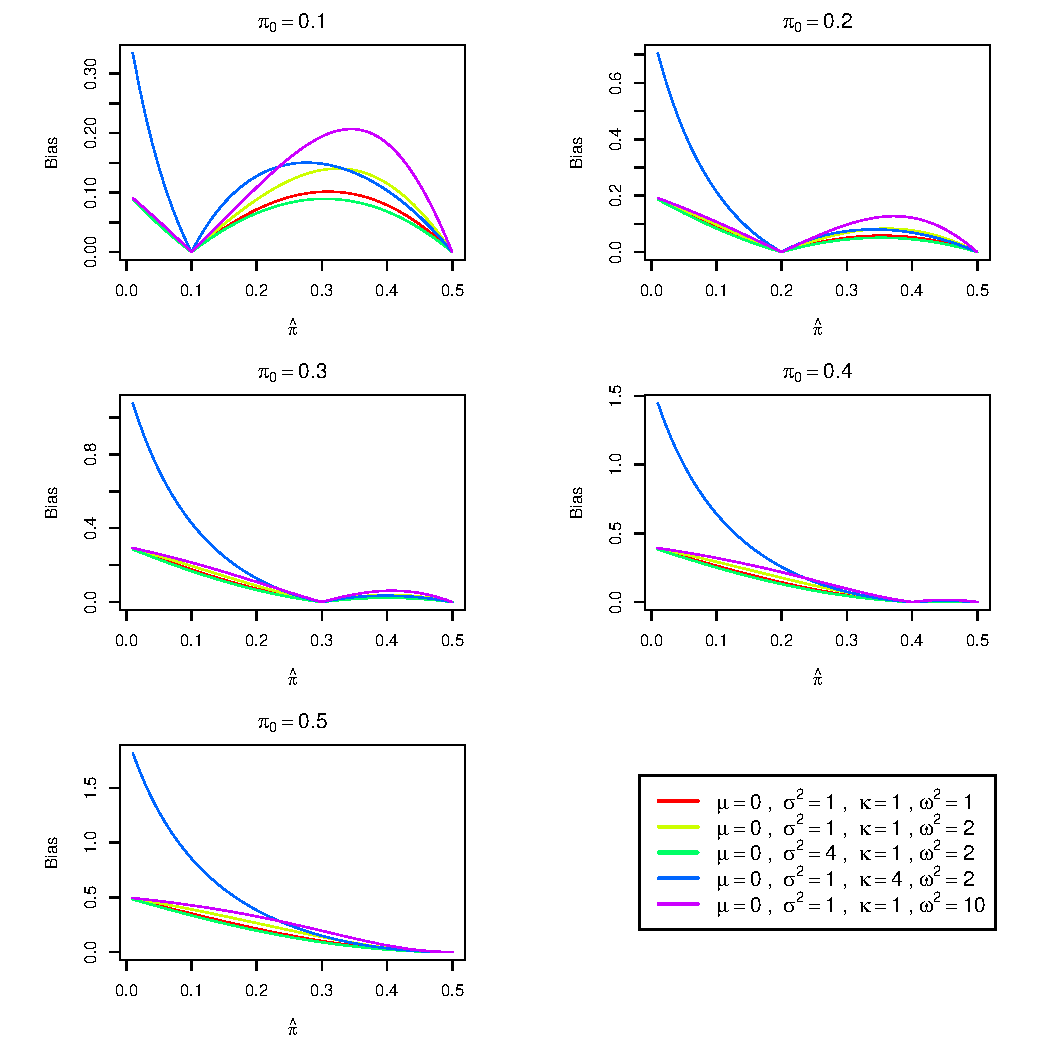
\includegraphics[width=\textwidth]{./Figures/bias_plot.pdf}
\label{bias_plot}
\end{center}
\end{figure}

\begin{figure}[htbp]
\begin{center}
\caption{Variance of $\hat{\mu}^*$ as a function of $\hat{\pi}$ with $N=1$}
\vspace{5pt}
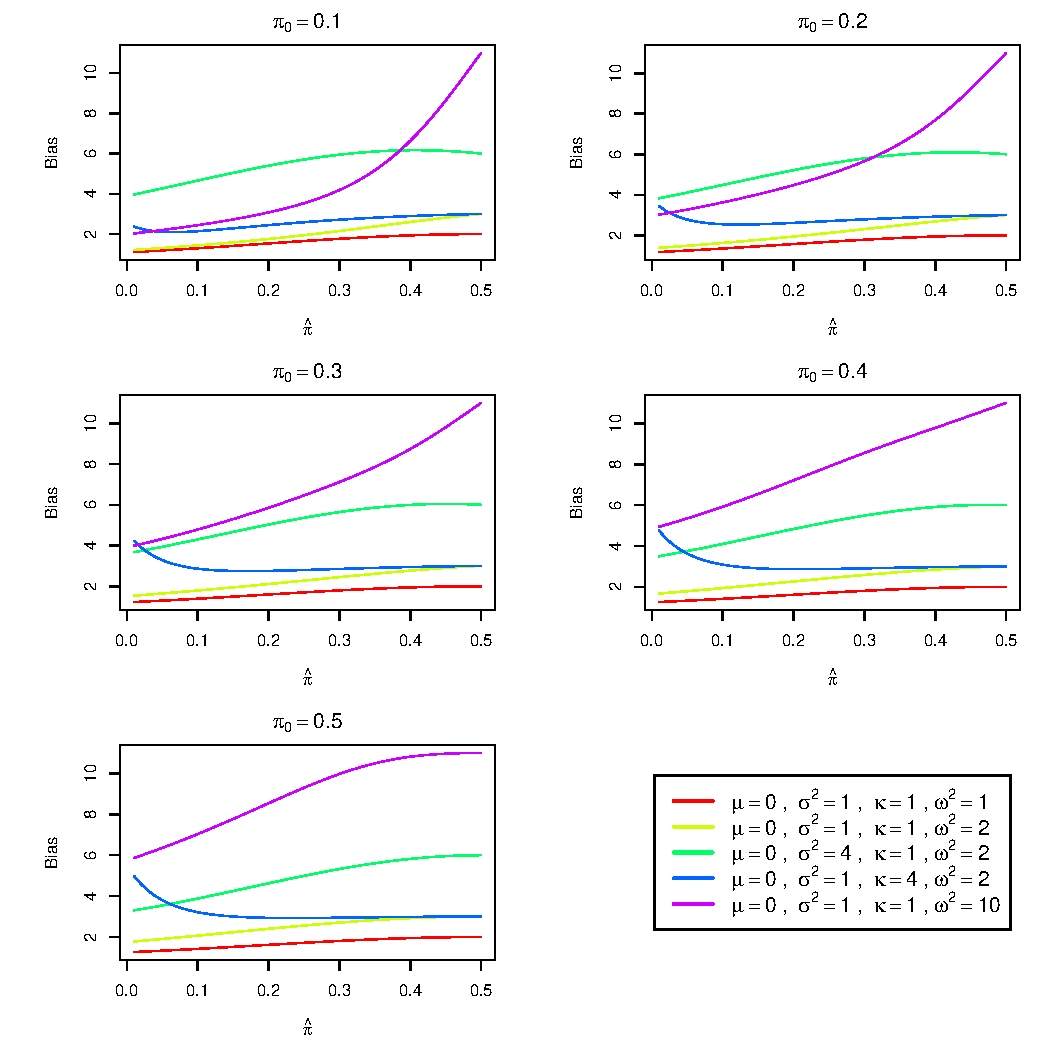
\includegraphics[width=\textwidth]{./Figures/var_plot.pdf}
\label{var_plot}
\end{center}
\end{figure}

% TO DO: Fix this but also try smaller deviations in $\hat{\pi}$!!!

For $N=1,000$, $\hat{\mu}^*$ only performs better when $\hat{\pi}=\pi$, and the benefits decrease as the true $\pi$ approaches 0.5.�  For $N=100$, the ratio is close to 1 for Bias($\hat{\pi}$) = 0.1, so that the efficiency gain from incorporating knowledge about $\pi$ is reduced for $N > 100$.  This suggests that for small samples, you may want to incorporate knowledge about probabilities; but for samples of a large size, it's best to ignore them and weight multiple matches equally. 

\begin{table}

\caption{\label{tab:}MSE ratio for $\hat{\mu}^*$ and $\hat{\mu}^{AHL}$ for $N=10$ and $(\mu, \sigma^2, \kappa, \omega^2) = ($0,1,1,2)}
\centering
\begin{tabular}[t]{cccccc}
\toprule
\multicolumn{1}{c}{ } & \multicolumn{5}{c}{$\hat{\pi}}$} \\
\cmidrule(l{3pt}r{3pt}){2-6}
$\pi$ & 0.1 & 0.2 & 0.3 & 0.4 & 0.5\\
\midrule
0.1 & 2.085 & 1.635 & 1.280 & 1.097 & 1\\
0.2 & 1.744 & 1.545 & 1.275 & 1.093 & 1\\
0.3 & 1.381 & 1.371 & 1.225 & 1.078 & 1\\
0.4 & 1.073 & 1.165 & 1.141 & 1.054 & 1\\
0.5 & 0.836 & 0.967 & 1.036 & 1.022 & 1\\
0.6 & 0.658 & 0.796 & 0.924 & 0.983 & 1\\
0.7 & 0.527 & 0.656 & 0.814 & 0.938 & 1\\
0.8 & 0.428 & 0.543 & 0.713 & 0.891 & 1\\
0.9 & 0.354 & 0.454 & 0.623 & 0.842 & 1\\
\bottomrule
\end{tabular}
\end{table}

\begin{table}

\caption{\label{tab:}MSE ratio for $\hat{\mu}^*$ and $\hat{\mu}^{AHL}$ for $N=100$ and $(\mu, \sigma^2, \kappa, \omega^2) = ($0,1,1,2)}
\centering
\begin{tabular}[t]{ccccccccccc}
\toprule
\multicolumn{1}{c}{ } & \multicolumn{10}{c}{$\hat{\pi}}$} \\
\cmidrule(l{3pt}r{3pt}){2-11}
$\pi$ & 0.05 & 0.1 & 0.15 & 0.2 & 0.25 & 0.3 & 0.35 & 0.4 & 0.45 & 0.5\\
\midrule
0.1 & 1.930 & 2.085 & 1.658 & 1.183 & 0.886 & 0.740 & 0.703 & 0.763 & 0.910 & 1\\
0.2 & 0.808 & 1.164 & 1.502 & 1.545 & 1.317 & 1.079 & 0.944 & 0.915 & 0.966 & 1\\
0.3 & 0.383 & 0.536 & 0.763 & 1.039 & 1.230 & 1.225 & 1.115 & 1.029 & 1.004 & 1\\
0.4 & 0.216 & 0.286 & 0.394 & 0.558 & 0.776 & 0.981 & 1.072 & 1.054 & 1.017 & 1\\
0.5 & 0.137 & 0.173 & 0.230 & 0.319 & 0.457 & 0.651 & 0.855 & 0.977 & 1.003 & 1\\
0.6 & 0.094 & 0.116 & 0.148 & 0.200 & 0.285 & 0.423 & 0.622 & 0.837 & 0.966 & 1\\
0.7 & 0.068 & 0.082 & 0.103 & 0.136 & 0.190 & 0.285 & 0.446 & 0.683 & 0.909 & 1\\
0.8 & 0.052 & 0.061 & 0.075 & 0.098 & 0.135 & 0.201 & 0.325 & 0.546 & 0.839 & 1\\
0.9 & 0.041 & 0.047 & 0.057 & 0.073 & 0.100 & 0.148 & 0.243 & 0.435 & 0.764 & 1\\
\bottomrule
\end{tabular}
\end{table}

\begin{table}

\caption{\label{tab:}MSE ratio for $\hat{\mu}^*$ and $\hat{\mu}^{AHL}$ for $N=1000$ and $(\mu, \sigma^2, \kappa, \omega^2) = ($0,1,1,2)}
\centering
\begin{tabular}[t]{cccccc}
\toprule
\multicolumn{1}{c}{ } & \multicolumn{5}{c}{$\hat{\pi}}$} \\
\cmidrule(l{3pt}r{3pt}){2-6}
$\pi$ & 0.1 & 0.2 & 0.3 & 0.4 & 0.5\\
\midrule
0.1 & 2.085 & 0.314 & 0.142 & 0.188 & 1\\
0.2 & 0.269 & 1.545 & 0.425 & 0.349 & 1\\
0.3 & 0.075 & 0.303 & 1.225 & 0.706 & 1\\
0.4 & 0.034 & 0.090 & 0.409 & 1.054 & 1\\
0.5 & 0.019 & 0.041 & 0.138 & 0.682 & 1\\
0.6 & 0.012 & 0.024 & 0.066 & 0.337 & 1\\
0.7 & 0.009 & 0.015 & 0.038 & 0.183 & 1\\
0.8 & 0.006 & 0.011 & 0.025 & 0.112 & 1\\
0.9 & 0.005 & 0.008 & 0.017 & 0.075 & 1\\
\bottomrule
\end{tabular}
\end{table}


\subsection{Incorporating $\pi$ in linear regression}

Suppose we have two matches $\{y_{i1}, y_{i2}\}_{i=1}^N$ for each observation.  We get the same conditions for unbiasedness of the OLS estimator if we consider using a linear combination of the $y$'s, as in the model:
\begin{equation} a_1 y_{i1} + a_2 y_{i2} - \kappa = x_i'\beta + \varepsilon_i, \ \hspace{10pt} \Var{\varepsilon | x_i } = \sigma^2  \end{equation}
Then the OLS estimator is
$$ \hat{\beta} = \left(\frac{1}{N}\sum_{i=1}^N x_i x_i'\right)^{-1} \left(\frac{1}{N}\sum_{i=1}^N x_i'(a_1 y_{i1} + a_2 y_{i2} - \kappa)\right) $$
and
\begin{align*}
E\left[\hat{\beta}\right] &= E[x_ix_i']^{-1} E[x_i'(a_1 y_{i1} + a_2 y_{i2} - \kappa] \\
&= \beta(a_1 \pi + a_2 (1-\pi)) + E[x_ix_i']^{-1}E[x_i](a_2 \pi + (1-\pi)a_1 - a_3) \kappa 
\end{align*}
Unbiasedness requires the same conditions on $a_1, a_2,$ and $a_3$ as derived in Lemma 1, i.e.
\begin{align*}
a_2(a_1) &=  \frac{1-\pi a_1}{1-\pi} \\ a_3(a_1) &= \frac{\pi}{1-\pi} + \frac{a_1 - 2\pi a_1}{1-\pi} 
\end{align*}
which means that any unbiased linear estimator $\hat{\beta}$ can be written as a linear combination of unbiased estimators that use only $y_{i1}$ or $y_{i2}$,
\begin{align*}
\hat{\beta}_{1} &= \left(\frac{1}{N}\sum_{i=1}^N x_i x_i'\right)^{-1}\frac{1}{N}\sum_{i=1}^N \frac{x_i y_{i1}}{\pi} - \frac{1-\pi}{\pi}\kappa \\
 \hat{\beta}_{2} &= \left(\frac{1}{N}\sum_{i=1}^N x_i x_i'\right)^{-1}\frac{1}{N}\sum_{i=1}^N \frac{x_i y_{i2}}{1-\pi} - \frac{\pi}{1-\pi}\kappa 
 \end{align*}
 and so the minimum variance estimator is $\hat{\beta}^* = d^* \hat{\beta}_1 + (1-d^*)\hat{\beta}_2$, where 
 \begin{equation}
 d^* = \frac{\Var{\hat{\beta}_{2}} - \text{Cov}\left(\hat{\beta}_1, \hat{\beta}_2\right)}{\Var{\hat{\beta}_1} + \Var{\hat{\beta}_{2}} - 2 \text{Cov}\left(\hat{\beta}_1, \hat{\beta}_2\right)}
 \end{equation}
and we can repeat the exercise in the previous sections, comparing variance and bias for misspecified beliefs $\hat{\pi}$ and different parameter combinations.  The choice of the weights $d^*$ that give the optimal $\hat{\beta}^*$ is now complicated by the fact that it depends on the second moments of $X_i$, however the formulas for $\Var{\hat{\beta}_i}$ are the same as in (\ref{vmu1})-(\ref{cov}), but replacing $\mu, \sigma^2, \kappa,$ and $\omega^2$ with: 

% add this here

\subsection{Generalizing results to $L_i > 2$}

% to do 

\section{Numerical Example}
In order to compare how the methods discussed in Sections 3 and 4 perform in practice, I conduct a Monte Carlo study using simulated data.  The purpose of this section is to introduce a numerical example that is representative of one observation in the Monte Carlo study.  The benefits of using simulated data is that I can control the degree of similarity among identifying variables, and overlap between datasets, all while knowing the true match status of each $(x_i,y_j)$ record pair.  As a result, I can compare how sensitive my results are to data quality, and compare how the various matching and estimation procedures perform relative to the correctly specified model applied to a  dataset containing only correct links.

I begin by constructing a ``ground truth" dataset with 1000 observations of $(x_{1i}, x_{2i}, y_i, w_i)$, where $x_{1i}$ and $x_{2i}$ are mutually independent, i.i.d draws from Bernoulli(0.5) and Normal(0,2) distributions, respectively.s  The $y_i$ values are generated according to \begin{gather}
y_i = \beta_0 + \beta_1 x_{1i} + \beta_2 x_{2i} + \varepsilon_i, \hspace{10pt} 
\varepsilon_i\  |\  x_{1i}, x_{2i} \overset{i.i.d}{\sim} \mathcal{N}(0, \sigma^2) 
\end{gather}
where $\varepsilon_i$ are independent draws from a Normal(0,2) distribution.  I chooses $(\beta_0, \beta_1, \beta_2, \sigma^2) = (2, 0.5, 1, 2)$, so that estimating the correctly specified linear regression model yields an $R^2$ value of approximately 0.50.  

The vector of identifying variables, $w_i$, includes a first name, last name, and birth year.  In total, there are 960 unique first and last name combinations, so multiple observations will be assigned the same first and last name.  The birth years are drawn at random from a uniform distribution over the set of integers between 1900 and 1925.  The resulting dataset resembles the top panel of Figure \ref{sample_dta}.  
 
 \begin{figure}[htbp]
\caption{Creation of Synthetic Datasets}
\vspace{5pt}
 \begin{adjustwidth}{-.5in}{-.5in}  
\begin{tikzpicture}
\node (a) at (0,0){
\begin{tabular}{ccccccc}
\toprule
ID &  $y$ & $x_1$ & $x_2$ & First Name & Last Name & Birthday \\
\midrule
1 & $y_1$ & $x_{1,1}$ & $x_{2,1}$ & Tyler & Ashenfelter & 1915-05-13 \\
2 & $y_2$ & $x_{1,2}$ & $x_{2,2}$ & Brandon & Christensen & 1904-06-27 \\
\mc{7}{c}\vdots \\
195 & $y_{195} $ &$x_{1,195} $& $x_{2,195}$ & Samantha & Andersen & 1914-08-18 \\
196 & $y_{196}$ & $x_{1,196}$& $x_{2,196}$ & Victoria & Andersen & 1918-11-25\\
\mc{7}{c}\vdots \\ 
1000 & $y_{500}$ & $x_{1,500}$ & $x_{2,500}$ & Vicky & Anderson & 1915-04-14\\
\bottomrule
\end{tabular}};
\\
\vspace{20pt}
\\
\footnotesize{
\node[yshift=-3cm] (b) at (a.south){
\begin{tabular}{ cc }   % top level tables, with 2 rows
$x$-Datafile & $y$-Datafile \\  
% bottom left of the top level table: table 1 
\begin{tabular}{ cccc } 
\toprule
ID & $x$ & Name & Birthday \\
\midrule
2 & ($x_{1,2}, x_{2,2})$ & Branden Christenson & 1905-06-27 \\
\mc{4}{c}\dots \\
195 & ($x_{1,195},x_{2,195}$)& Samantha Anderson & 1914-08-21 \\
198 & ($x_{1,198}, x_{2,198}$)& Jon Smyth & 1918-12-20\\
\mc{4}{c}\dots \\ 
1000 & ($x_{1,1000},x_{2,1000}$) & Vic Andersn & 1915-04-14\\
\bottomrule
\end{tabular} &  % starting bottom right of the top level table
% table 2
\begin{tabular}{ cccc } 
\toprule
ID & $y$ & Name & Birthday \\
\midrule
1 & $y_1$ & Tyler Ashenfelter & 1915-05-13 \\
2 & $y_2$ & Brandon Christensen & 1904-06-27 \\
\mc{4}{c}\dots \\
195 & $y_{1,195}$ & Samantha Anderson & 1914-08-18 \\
\mc{4}{c}\dots \\ 
1000 & $y_{1000}$ & Vicky Anderson & 1915-04-14\\
\bottomrule
\end{tabular} \\
\end{tabular}};
\draw[->, thick](a)--(b);
\end{tikzpicture}
\end{adjustwidth}
\label{sample_dta}
\end{figure}%


 
 % Massive latex Figure of synthetic dataset -- put in new file ideally
Next, I split the ground truth dataset into the $x$- and $y$-datafiles, as in the bottom panel of Figure \ref{sample_dta}.  The $x$-datafile contains values of $(x_{i1},x_{i2})$ for 500 observations selected at random from the ground truth dataset.  The identifiers in the $x$-datafile are equal to the original $w_i$ plus some random transcription error.  The probability of introducing a certain type ofs typographical error is equal to that reported for the 1940 Census data in \cite{abe2019}\foonote{For example, 7\% of observations have misreported first names and 17\% of observations have misreported last names.} These errors include deleting characters (e.g., ``Anderson"  becomes ``Andersn"), exchanging vowels (e.g., ``Rachel" becomes ``Rachal"), and swapping English phonetic equivalents (e.g. ``Ellie" becomes ``Elie").  For half of the observations, I introduce random errors in the birth year drawn from a Normal(0, 2.5) distribution and rounded to the nearest integer.  

The $y$-datafile includes all 1,000 values of $y_i$ from the ground truth data, along with the original identifiers $w_i$.  The aim of this construction is to make it likely that some observations in the $x$-datafile will be linked to multiple values of $y$.  The next section describes the record linkage methods used to link the $x$- and $y$-datafiles. 

\section{Record Linkage Methods}

Recall that the data consist of an $x$-datafile, denoted $X \equiv \{(x_i, w_i): i  = 1,\dots,N_x \}$, and a $y$-datafile, denoted $Y \equiv \{(y_j,w_j): j = 1, \dots, N_y\}$, and the goal of record linkage is to use $w_i$ and $w_j$ to determine which $i \in \{1, \dots, N_x\}$ and $j \in \{1, \dots, N_y\}$ refer to the same individual.  

For the purposes of this paper, I define a record linkage procedure as a set of decisions about (i) selecting and standardizing the identifying variables in $w_i$ and $w_j$, (ii) choosing which $(i,j)$ pairs to consider as potential matches, (iii) defining which patterns of $(w_i,w_j)$ constitute (partial) agreements, and (iv) designating $(i,j)$ pairs as matches.\footnote{By contrast, \cite{bailey2017} categorize record linkage procedures according to the set of assumptions that motivate their use.}  

Step (i) addresses the fact that differences may arise in $w_i$ and $w_j$ because of transcription error or misreporting, even when observations $i$ and $j$ refer to the same individual.   In practice, this step consists of removing spaces and non-alphabetic characters from string variables and processing names with phonetic algorithms to account for potential misspellings; common nicknames may also be replaced with full names.  

Step (ii) reduces the computational burden of a matching procedure when $N_x \times N_y$ is large by partitioning $X\times Y$ into ``blocks."  Only records within the same block are attempted to be matched, while records in different blocks are assumed to be non-matches.  Blocking variables should be recorded with minimal error, otherwise blocking may adversely affect the Type II error rate. 

Step (iii) defines a metric for quantifying the similarity between non-numeric variables, such as Jaro-Winkler distances for strings.  For more details, see \cite{arp2018}. 

Finally, Step (iv) is where record linkage procedures differ in the most meaningful ways; hence, this step will be the focus of my analysis.  Consider the following (deterministic) record linkage procedure as an example:
\begin{enumerate}
\item[(i)] Use a phonetic algorithm to standardize the first and last names in both datasets; 
\item[(ii)] Consider as potential matches all $(i, j)$ pairs whose phonetically standardized names begin with the same letter, and whose birth years are within $\pm$2 years;
\item[(iii)] Measure the distance between any two names using Jaro-Winkler string distance, and the distance between any two birth dates as a difference in months;
\item[(iv)] Designate as matches all $(i,j)$ pairs with Jaro-Winkler scores exceeding a pre-determined cut-off; and, if a record $i$ has multiple possible matches that exceed the cut-off, then choose the corresponding $j$ with the highest score (or pick one match at random if there is a tie).  
\end{enumerate}
Another record linkage procedure could be defined using the same steps (i)-(iii), but replacing (iv) with a probabilistic matching rule that does not enforce one-to-one matching:
\begin{enumerate}
\item[(iv*)]  Use the Expectation-Maximization algorithm to compute ``match weights" for each $(i,j)$ pair; then, designate as matches all pairs with match weights exceeding a threshold that is set to reflect specific tolerances for Type I and Type II error. 
\end{enumerate} 

Except in rare cases, the estimated matching functions obtained by switching (iv) and (iv$^*$) will differ, if only because the former method matches each $x$ with at most one $y$, the latter potentially matches the same $x$ with multiple $y$.  This example also illustrates the difference between deterministic and probabilistic record linkage methods: while (iv) uses pre-determined rules to designate pairs as matches, (iv*) uses statistical theory to inform the selection of the decision rule.  Probabilistic record linkage also involves the estimation of match weights, which can be incorporated in subsequent estimation steps.

Below I will discuss two record linkage methods -- one deterministic and one probabilistic -- that I will use in my analysis.  Each method will be implemented twice: first, requiring unique matches, and then allowing for multiple matches.  While these methods are by no means exhaustive, they are intended to be representative of the most commonly used methods in economics.  For a detailed survey of record linkage techniques, please refer to books by \cite{harron_book, christen2012} or \cite{herzog07}, or any of the references in this paper. 

\subsection{Deterministic}
The deterministic matching algorithm described herein is based upon methods developed by \cite{abe2012}.  It consists of the following steps.
\begin{enumerate}
\item Clean names in the $x$- and $y$- datafiles to remove any non-alphabetic characters and account for common mis-spellings and nicknames (e.g., so that Ben and Benjamin would be considered the same name).  
\item Restrict the sample to people in the $x$-datafile with unique first name, last name, and birth year combinations  
\item For each record in the $x$-datafile, look for records in the $y$-datafile that match on first name, last name, place of birth, and exact birth year.  At this point there are three possibilities 
\begin{enumerate}
\item If there is a \textit{unique} match, this pair of observations is considered a match.
\item If there are multiple potential matches in the $y$-datafile with the same year of birth, the observation is discarded. 
\item If there are no matches by exact year of birth, the algorithm searches for matches within $\pm$ 1 year of reported birth year, and if this is unsuccessful, it looks for matches within $\pm$ 2 years.  In each of these steps, only unique matches are accepted.  If none of these attempts produces a unique match, the observation is discarded.
\end{enumerate}
\item Repeat Step 3 for each record in the $y$-datafile, searching for matches in the $x$-datafile; then designate as matches all record pairs in the intersection of the two matched samples.
\end{enumerate}

An interesting quirk of this algorithm is that an individual with multiple matches is dropped from the sample only if those matches occur before a unique match is found in Step 3.  That is, a person with a unique, same-year match, and multiple matches with birth years within one year, will not be dropped from the sample.  If the same-year match were not included in the dataset, then that same individual would be dropped.  This has significant implications for bootstrapping standard errors; notably, the nonparametric bootstrap will fail. 

Note that this quirk only occurs when the algorithm enforces unique matches.  When allowing for multiple matches, I designate as a match any pair that satisfies any of the categories in Step 3. 

\subsection{Probabilistic Record Linkage}
The probabilistic record linkage technique implemented in this paper is based on the canonical model by \cite{fellegi69}, which views record linkage as a classification problem, where every record pair belongs either to the set of \textit{matches} $(M)$ or \textit{non-matches} $(U)$:
\begin{align*} M &= \{ (i,j) \in X\times Y: j \in \varphi(i) \} \\ U &= \{(i,j) \in X\times Y:  j \notin\varphi(i)\}\end{align*} 

 To determine whether a record pair $(i,j)$ belongs to $M$ or $U$, the pair is evaluated according to $K$ different comparison criteria.  These comparisons are represented in a \textit{comparison vector}, $$\mathbf{\gamma_{ij}}= (\gamma_{ij}^1, \dots, \gamma_{ij}^{k}, \dots, \gamma_{ij}^K)$$  where each comparison field $\gamma_{ij}^{k}$ may be binary-valued, as in ``$i$ and $j$ have the same birthday" and ``$i$ and $j$ have the same last name," or use ordinal values to indicate partial agreement between strings.

The probability of observing a particular configuration of $\gamij$ can be modeled as arising from the mixture distribution:
\begin{equation}
P(\gamij) = P(\gamij | M) p_M + P(\gamij | U) p_U 
\label{mm}
\end{equation}
where $P(\gamij | M)$ and $P(\gamij | U)$ are the probabilities of observing the pattern $\gamij$ conditional on the record pair $(i,j)$ belonging to $M$ or $U$, respectively.  The proportions $p_M$ and $p_U = 1-p_M$ are the marginal probabilities of observing a matched or unmatched pair.  Applying Bayes' Rule, we obtain the probability of $(i,j) \in M$ conditional on observing $\gamij$,
\begin{equation} P(M | \gamij) = \frac{p_M P(\gamij | M)}{P(\gamij)} \label{bayes} \end{equation}
Thus, if we can estimate $p_M$, $P(\gamij | M)$ and $P(\gamij | U)$, then we can estimate the probability that any two records refer to the same entity using (\ref{bayes}).   These probabilities can then be used to designate pairs as matches, or to estimate the false positive rate associated with a particular match configuration using the formulas in \cite{fellegi69}.  

One difficulty arises from the fact that there are at least $2^K -1$ possible configurations of $\gamij$\footnote{There are more, if any of the comparison criteria are non-binary}.  While in principle we could model $P(\gamij | M)$ and $P(\gamij | U)$ as
\begin{align*} (\gamma_{ij}^1, \dots, \gamma_{ij}^K) \  |\  M &\sim \text{Dirichlet}(\mathbf{\delta_M})\\
 (\gamma_{ij}^1, \dots, \gamma_{ij}^K) \  |\  U &\sim \text{Dirichlet}(\mathbf{\delta_U}) \end{align*}
but the parameters $\mathbf{\delta_M}$ and $\mathbf{\delta_U}$ may be high-dimensional.  However, if the comparison fields $\gamma_{ij}^{k}$ are independent across $k$ conditional on match status, then the number of parameters used to describe each mixture class can be reduced to $K$ by factoring:
 \begin{equation} 
 P(\gamma_{ij} | C) = \prod_{k=1}^K P(\gamma_{ij}^{k} | C)^{\gamma_{ij}^{k}}(1-Pr(\gamma_{ij}^{k} | C))^{1-\gamma_{ij}^{k}} \hspace{20pt} C\in \{M, U\} 
 \label{eq:condInd}
 \end{equation}
 Alternatively, dependence between fields can be modeled using log-linear models; however, I will assume conditional independence to ease computation, and because the matching variables in the synthetic dataset are generated independently of each other.  
 
Since membership to $M$ or $U$ is not actually observed, a convenient way of simultaneously estimating $p_M, p_U$ and classifying record pairs as matches or non-matches is via mixture modeling, with mixture distributions $P(\gamij | M)$ and $P(\gamij | U)$.  The parameters can be estimated using the expectation-maximization (EM), first applied to record linakge by \cite{larsen_rubin_2001}.  For this paper, I use the \texttt{fastLink} algorithm developed by \cite{enamorado2019}. 




%\begin{align*}
%\Var{\hat{\mu}_1} &= \frac{1}{N}\Var{x_i y_{i1}} = \frac{1}{N}\frac{1}{\pi^2}\left(\pi \Var{x_i\varepsilon_i} + (1-\pi) \Var{x_i}\omega^2 + \pi(1-\pi)(E[x_i^2\beta] - E[x_i]\kappa)^2\right) \\
 %\hat{\mu}_2 &= \frac{1}{N}\sum_{i=1}^N \frac{x_i y_{i2}}{1-\pi} - \frac{\pi}{1-\pi}\kappa 
 %\end{align*}

%When performing estimation with linked data, a few obvious comparison metrics arise:  data can be partitioned into three parts - identfied links, nonlinks and potential links.  Could repeat the analysis for each group or for subsets of these groups.  They use nonlinks to adjust the potential links, and thereby, gain an additional perspective that could lead to reductions in MSE over statistics calculated only from the linked data.  Benchmark is OLS with one-to-one-matching, or using observations assigned $L_i = 1$ matches. 

%Using only data from pairs of records that are highly likely to be links might mean throwing away additional information from potentiallyl inked pairs, which could contain true links.  Additionally, we could bias results because confidently linked pairs may differ from potentially linked piars.  For example, considering affirmative actiona nd income questison, certain records may be harder to match.  For deterministic methods, people reweight on observables.. 

%Some methods specifically attempt to correct for the bias introduced by the matching step.  Seminal work by Neter, Maynes and Ramanathan (1965) shows that if matching errors are moderate then regression coefficeints can be severely biased.  This work is formalized by \cite{sw1993}. 


%The primary examples are \cite{lahiri05} and \cite{sw1993}.  \cite{sw1993} presuppose that the linker has provided a combined data file consisting of pairs of records (one from each input file) along with the match probability and the link status -- either link, nonlink, or potential link -- of each pair.  They assume that the file of linked cases has been augmented so that every record on the smaller of the two files has been paired with two records of the larger file having the highest matching weights.  Some cases will consist of (link, nonlink) combinations or (nonlink, nonlink) combinations, but they rule out settings where more than one true link could occur, so that (link link) combinations are ruled out.


\section{Monte Carlo Study}

Following the same procedure for simulating the empirical example described in Section 2, I generate 1,000 random $x$- and $y$- dataset pairs.  I implement four types of matching procedures using each dataset pair: (i) deterministic matching with unique matches (ABE Single), (ii) deterministic matching with multiple matches (ABE Multi), (iii) probabilistic matching with unique matches (PRL Single), and (iv) probabilistic matching with multiple matches (PRL Multi).  Allowing for multiple matches means that a single observation in the $x$- datafile may be matched to multiple observations in the $y$-datafile.  

Each matching method produces a distinct matched dataset, so that the matching step produces a total of 4,000 linked datasets.  Using each of the linked datasets, I then compute (i) naive OLS estimator (using all observations and also with observations assigned $(L_i=1)$, (ii) the \cite{sw1993} bias-corrected estimator, and (iii)  the AHL estimator that assigns equal weights to multiple matches.  As a benchmark, I also compute the OLS estimator that uses only the correctly matched pairs produced by the matching algorithm, and the OLS estimator applied to all 500 correctly linked record pairs.  Details on the implementation of these algorithms and estimation procedures can be found in the appendix.  

% Match Rate Table 

\begin{table}[htbp]
\let\center\empty
\let\endcenter\relax
\centering
\caption{Summary of matching algorithm performance}
\vspace{10pt}
\resizebox{\textwidth}{!}{
\begin{tabular}{cccccc}
\toprule
Method & Match Rate & \# Matches & Type I & Type II & P(Contains True)\\
\midrule
ABE (Single) & 0.71 (0.02) & 356.50 (10.60) & 0.03 (0.01) & 0.26 (0.02) & 0.97 (0.01)\\
ABE (Multi) & 0.79 (0.02) & 505.08 (17.30) & 0.23 (0.02) & 0.20 (0.02) & 0.99 (0.01)\\
PRL (Single) & 0.74 (0.02) & 369.15 (9.65) & 0.11 (0.02) & 0.15 (0.03) & 0.89 (0.02)\\
PRL (Multi) & 0.74 (0.02) & 435.65 (14.94) & 0.18 (0.02) & 0.23 (0.02) & 0.97 (0.01)\\
\bottomrule
\end{tabular}
}
\label{match_rate}
\end{table}

\begin{table}[htbp]
\let\center\empty
\let\endcenter\relax
\centering
\caption{Performance of multiple match methods by value of $L_i$}
\vspace{10pt}
\resizebox{\textwidth}{!}{
\begin{tabular}{lcccccc}
\toprule
L & 1 & 2 & 3 & 4 & 5 & 6+\\
\midrule
\addlinespace[0.3em]
\multicolumn{7}{l}{\textbf{ABE Multi}}\\
\hspace{1em}Pr(Contains True) & 0.99 (0.01) & 0.99 (0.01) & 0.99 (0.02) & 0.99 (0.07) & 0.99 (0.10) & 1.00 (0.00)\\
\hspace{1em}Pr(L=$\ell$) & 0.52 (0.15) & 0.35 (0.16) & 0.11 (0.11) & 0.03 (0.03) & 0.02 (0.03) & 0.02 (0.01)\\
\addlinespace[0.3em]
\multicolumn{7}{l}{\textbf{PRL Multi}}\\
\hspace{1em}Pr(Contains True) & 0.97 (0.01) & 0.98 (0.02) & 0.98 (0.06) & 0.98 (0.12) & 0.99 (0.05) & 1.00 (0.00)\\
\hspace{1em}Pr(L=$\ell$) & 0.59 (0.21) & 0.33 (0.22) & 0.07 (0.11) & 0.02 (0.05) & 0.03 (0.06) & 0.01 (0.01)\\
\bottomrule
\multicolumn{7}{l}{\textit{Note: } Based on 1,000 simulations. Standard deviations are reported in parentheses.}\\
\end{tabular}
}
\label{multi_L}
\end{table}

\subsection{Matching results}
To evaluate the matching procedures, I compute the following statistics for each linked dataset, reported in Table \ref{match_rate}:

\begin{itemize}
\item the proportion of observations in the $x$-datafile that are linked to at least one observation in the $y$-datafile (match rate), 
\item the total number of links made by the matching algorithm, 
\item the proportion of links that are incorrect (Type I error rate), 
\item the proportion of correct $(x,y)$ links that are not found by the matching algorithm (Type II error rate), 
\item the proportion of observations whose links include the true match
\end{itemize}

\noindent For the linked datasets that contain multiple matches per observation, I report also the average number of links per observation, and how often those links include the true match (Table \ref{multi_L}). 

%  Match Rate Histograms 
\begin{figure}[htbp]
\begin{center}
\caption{Match Rates by Linking Procedure } 
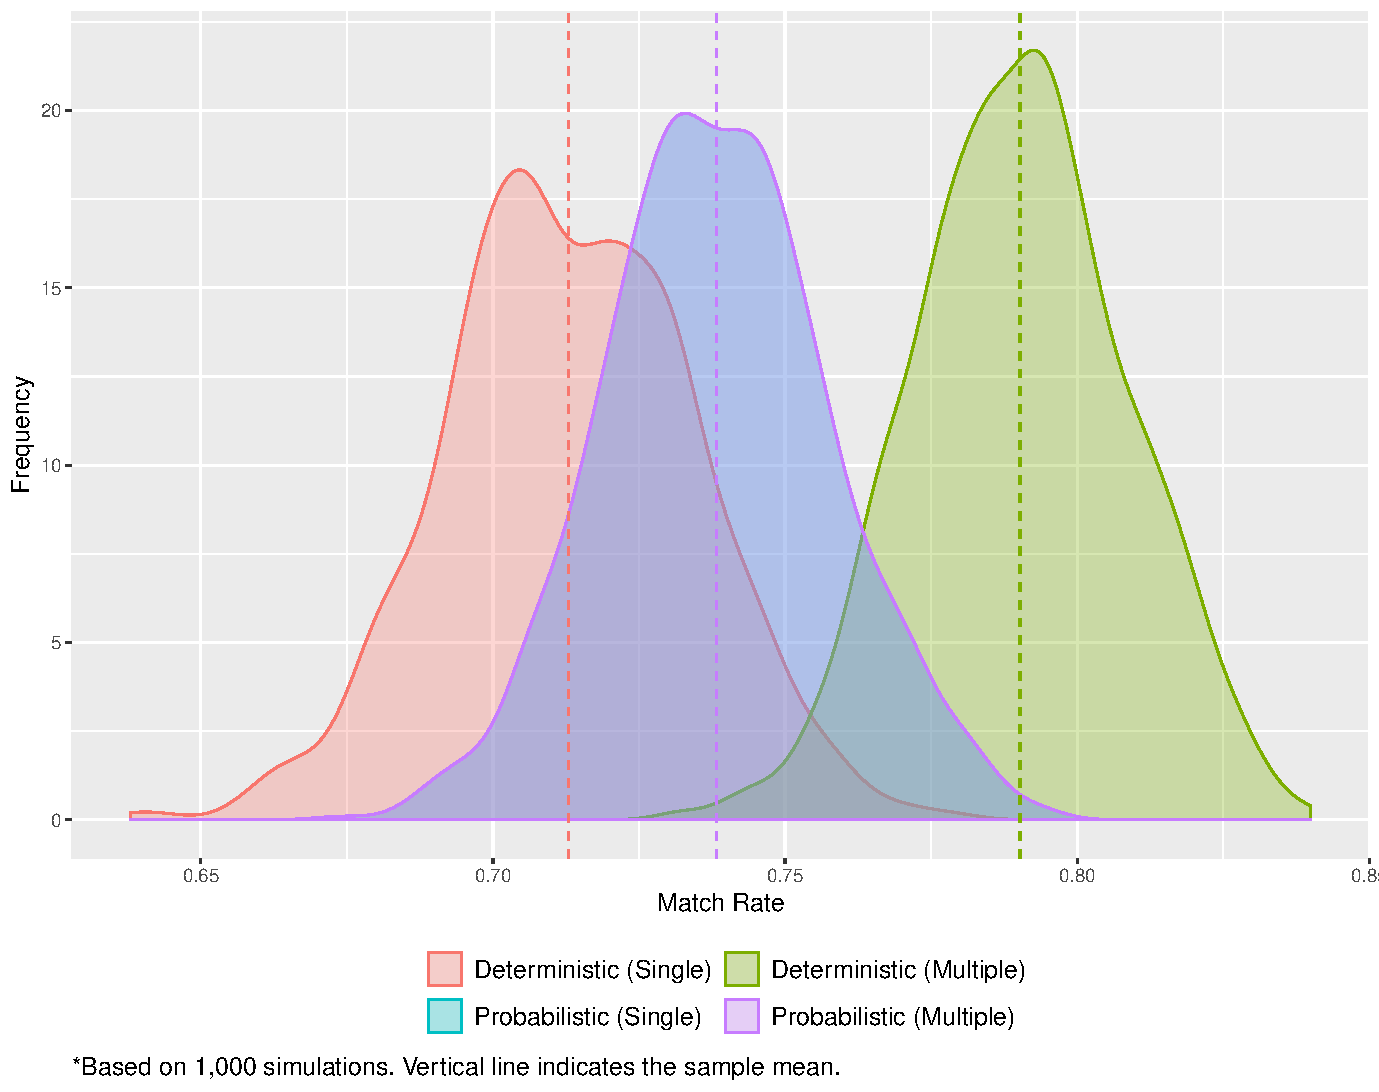
\includegraphics[width=0.9\textwidth]{./Figures/match_rate.pdf}
\label{match_hist}
\end{center}
\end{figure}

As seen in Table \ref{match_rate}, the average match rates range between 71 and 79 percent across the various matching procedures, but plotting the distribution of match rates in Figure \ref{match_hist}�shows that ABE Multi consistently matches more observations than any other procedure.  PRL Single and PRL Multi have about the same match rate, which suggests that allowing for multiple matches adds additional matches per observations rather than matching new individuals (however, this may be an artifact of how my PRL implementation).  ABE Multi, on the other hand, seems to increase match rates by matching new observations relative to ABE Single.  

When comparing Type I error rates, it is important to note that multiple-match methods will produce more false links by construction.  Therefore, it is best to compare multi-match methods by measuring the proportion of observations whose  matches contain the true link.  In this metric, both ABE Multi and PRL Multi perform very well.  Furthermore, we can compute these values for each value of $L_i$, as in Table \ref{multi_L}, which shows that allowing multiple matches improves the accuracy of the ABE algorithm.  Table \ref{multi_L} also shows that ABE Multi and PRL Multi rarely assign more than three matches to any given observation.  

Comparing ABE Single and PRL Single in Table \ref{match_rate}, demonstrates the  usual tradeoff between Type I and Type II errors.  ABE Single is more conservative, produces incorrect matches only 3 percent of the time, but failing to identify 26 percent of all matches.  PRL Single is less conservative, missing only 15 percent of matches, but at the cost of matching false links 11 percent of the time.    

Based on these results, ABE Multi seems to perform well if multiple matches are desired.  The linked datasets produced by ABE Multi are very likely to include the true match, which is required for all of the estimation methods described in this paper.  It is also easier in terms of computation, because it does not require linear sum assignment programs or thresholds to determine which record pairs should be designated as matches.  

\subsection{Estimation Results}

I compare the estimators according to median absolute deviation, and plot histograms of the estimated values in Figures \ref{olstrue}-\ref{ols}.  In implementing the AHL (2019) estimator, I set $\hat{g}(w_i, L_i) = \sum_{j=1}^{N_y} y_j $, the mean of all $y$ observations, to reduce the computational burden and because I have generated $y$ such that it is independent of the identifiers $w_i$.  The AHL estimator will probably perform better in scenarios where $w_i$ has predictive power in estimating the conditional mean of $y_i$.   



\begin{table}[h!]
\let\center\empty
\let\endcenter\relax
\centering
\caption{Median Absolute Deviations for Estimators}
\vspace{10pt}
\resizebox{0.9\textwidth}{!}{
\begin{tabular}{>{\raggedright\arraybackslash}p{5cm}ccccc}
\toprule
Parameter & AHL & SW & NaiveOLS & OLSTrue & OLS(L=1)\\
\midrule
\addlinespace[0.3em]
\multicolumn{6}{l}{\textbf{ABE Single}}\\
\hspace{1em}$\beta_0$ & 0.113 & 0.113 & 0.113 & 0.109 & 0.113\\
\hspace{1em}$\beta_1$ & 0.150 & 0.150 & 0.150 & 0.152 & 0.150\\
\hspace{1em}$\beta_2$ & 0.057 & 0.057 & 0.057 & 0.054 & 0.057\\
\addlinespace[0.3em]
\multicolumn{6}{l}{\textbf{ABE Multi}}\\
\hspace{1em}$\beta_0$ & 0.115 & 0.155 & 0.103 & 0.100 & 0.120\\
\hspace{1em}$\beta_1$ & 0.155 & 0.201 & 0.149 & 0.148 & 0.159\\
\hspace{1em}$\beta_2$ & 0.055 & 0.077 & 0.064 & 0.050 & 0.061\\
\addlinespace[0.3em]
\multicolumn{6}{l}{\textbf{PRL Single}}\\
\hspace{1em}$\beta_0$ & 0.115 & 0.115 & 0.115 & 0.112 & 0.115\\
\hspace{1em}$\beta_1$ & 0.163 & 0.163 & 0.163 & 0.162 & 0.163\\
\hspace{1em}$\beta_2$ & 0.063 & 0.063 & 0.063 & 0.056 & 0.063\\
\addlinespace[0.3em]
\multicolumn{6}{l}{\textbf{PRL Multi}}\\
\hspace{1em}$\beta_0$ & 0.116 & 0.150 & 0.112 & 0.106 & 0.123\\
\hspace{1em}$\beta_1$ & 0.168 & 0.204 & 0.165 & 0.158 & 0.175\\
\hspace{1em}$\beta_2$ & 0.058 & 0.074 & 0.062 & 0.055 & 0.064\\
\bottomrule
\end{tabular}
}
\label{multi_tab}
\end{table}

\begin{figure}[htbp]
\begin{center}
\caption{Comparing OLS with true matches produced by matching algorithm vs. matches with L=1}
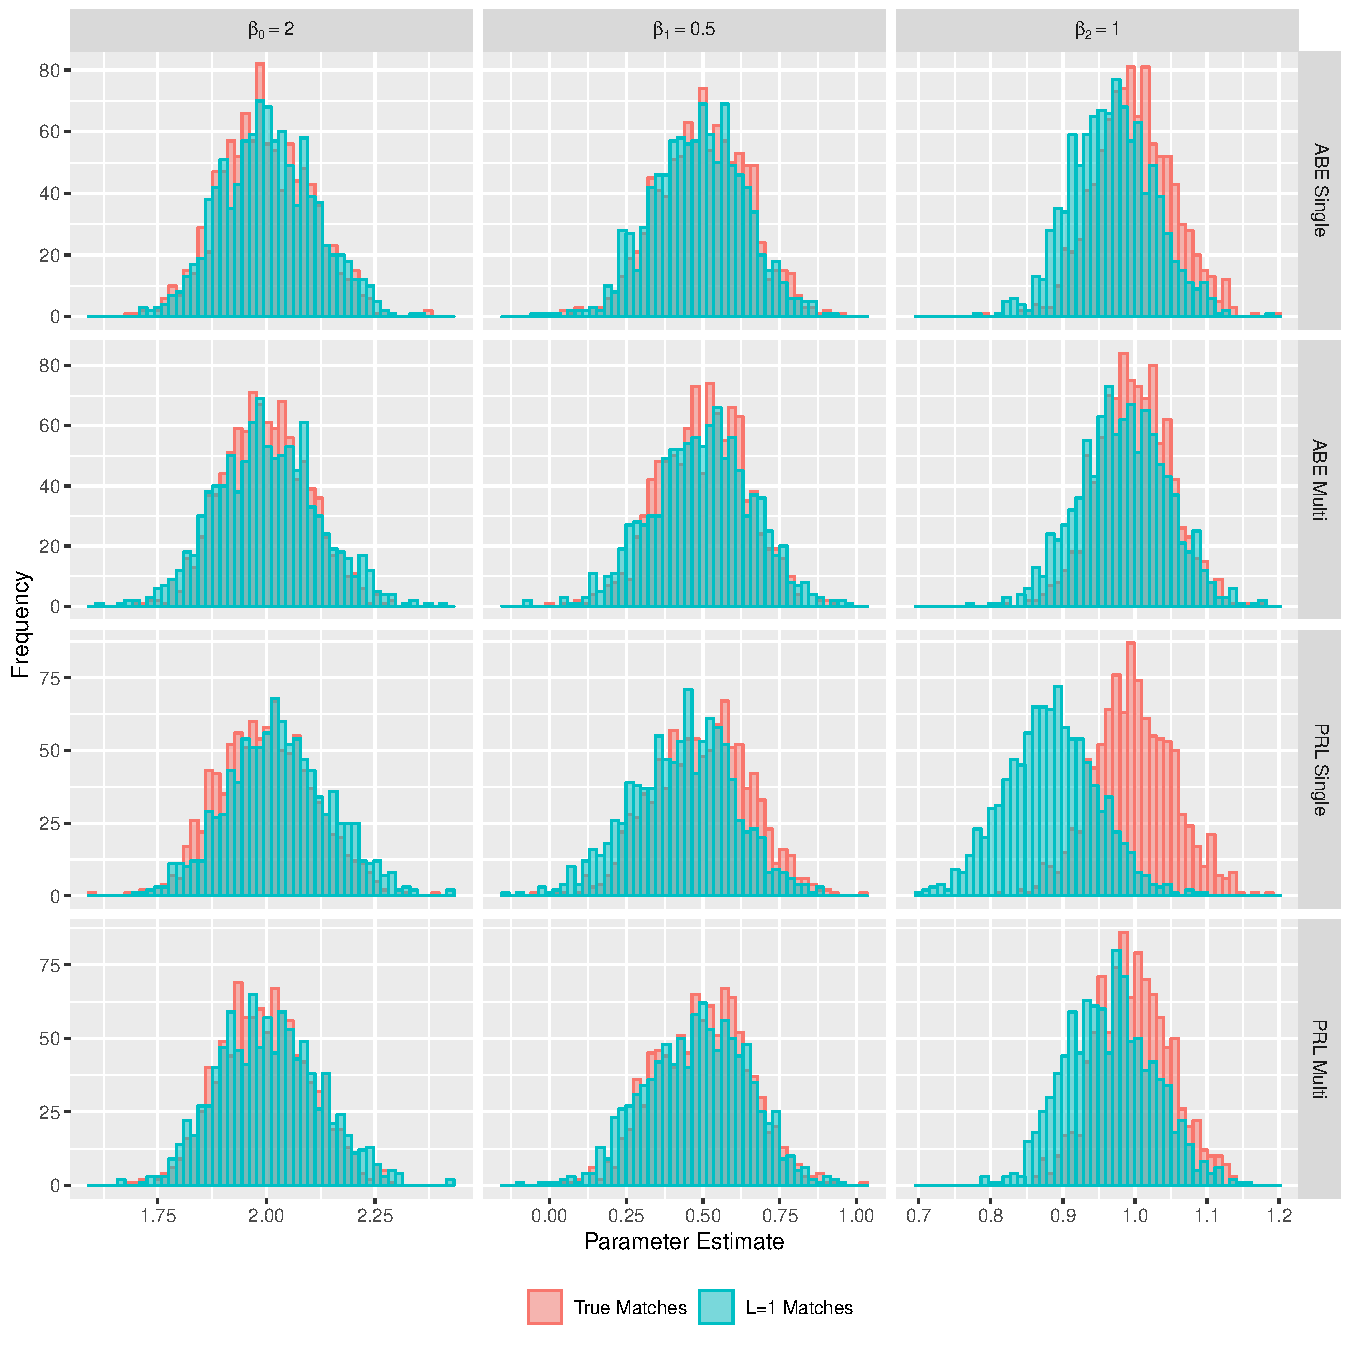
\includegraphics[width=1.1\textwidth]{./Figures/compare.pdf}
\label{olstrue}
\end{center}
\end{figure}


\section{Discussion/Conclusion}
To what extent my results generalize beyond the simulated data is unclear, as I made many arbitrary choices while generating the synthetic data -- such as the dictionary of names and the structure of the typographical errors that I introduce in the $x$-datafile -- that may impact my results in important ways.  However, my theoretical results suggest that (i) using the match that is most likely to be correct, and bias correcting based on the probability that it is correct is optimal, (ii) if weights are estimated imprecisely, or if no match has a high probability of being correct, then the it is better to assign equal weights to multiple matches.   This result needs to be studied using more general models, and ideally applied to real data.




% distribution of estimators
\begin{figure}[htbp]
\label{ahl_hist}
\begin{center}
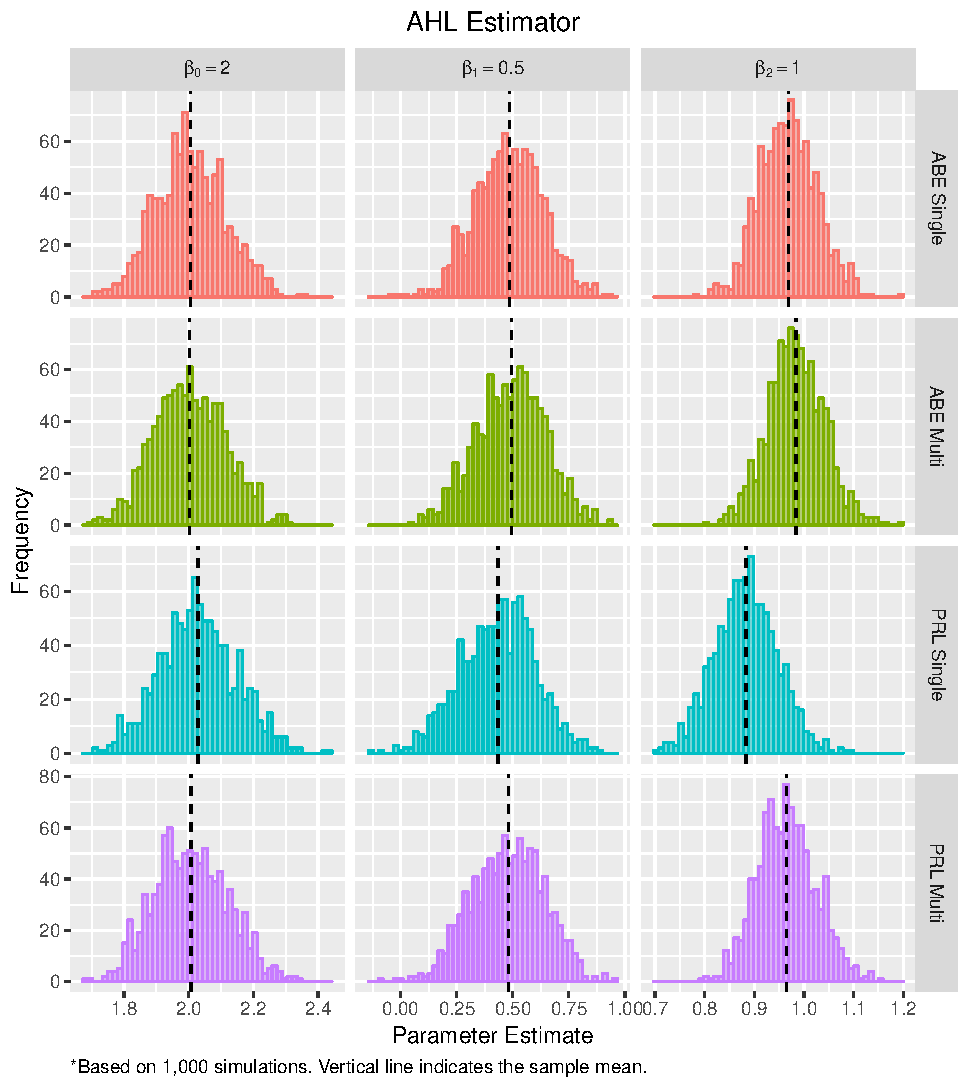
\includegraphics[width=\textwidth]{./Figures/ahl_hist.pdf}
\label{ahl}
\end{center}
\end{figure}

\begin{figure}[htbp]
\label{sw_hist}
\begin{center}
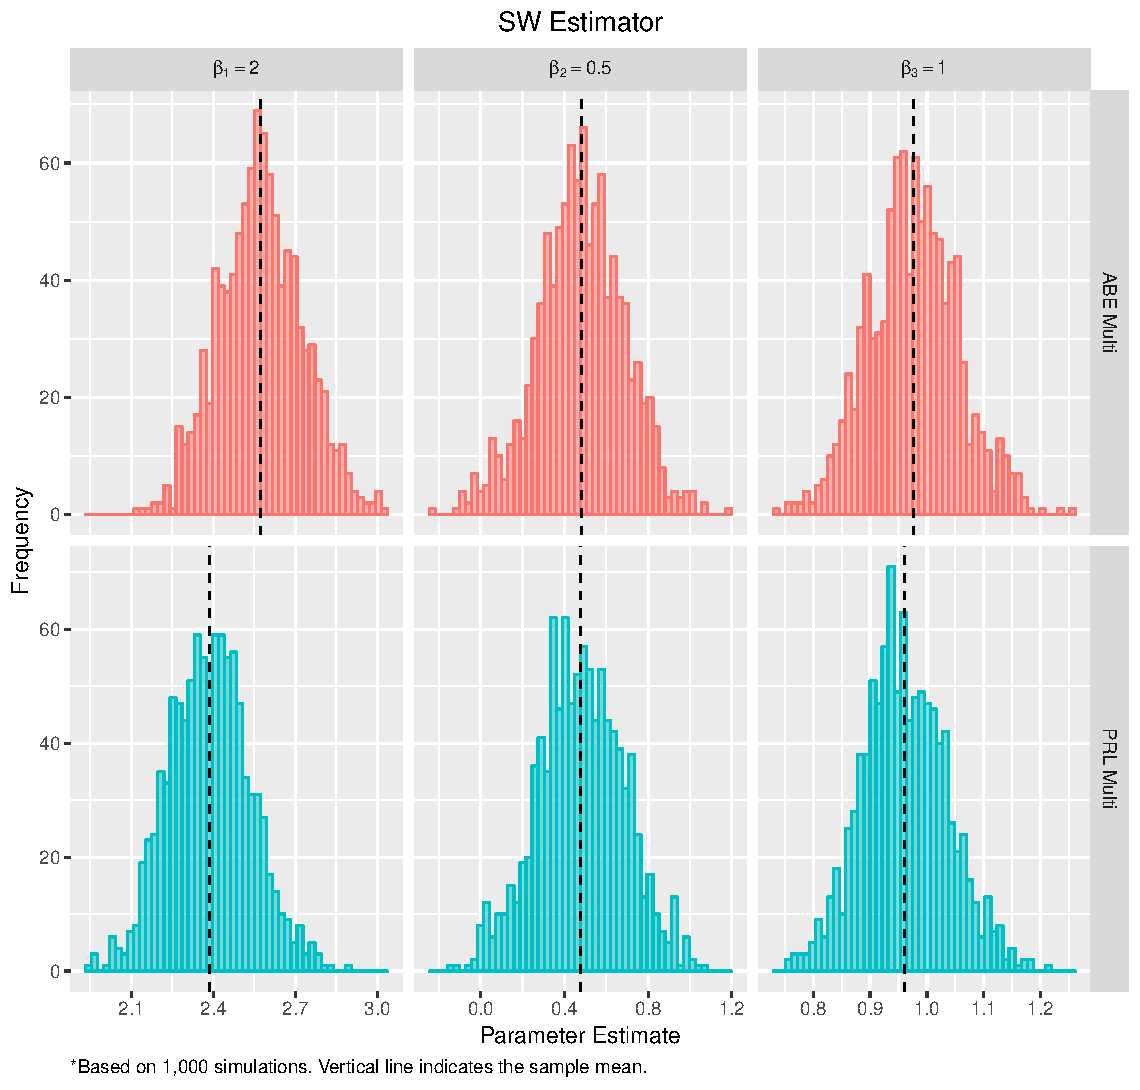
\includegraphics[width=\textwidth]{./Figures/sw_hist.pdf}
\label{sw}
\end{center}
\end{figure}


\begin{figure}[htbp]
\label{ols_hist}
\begin{center}
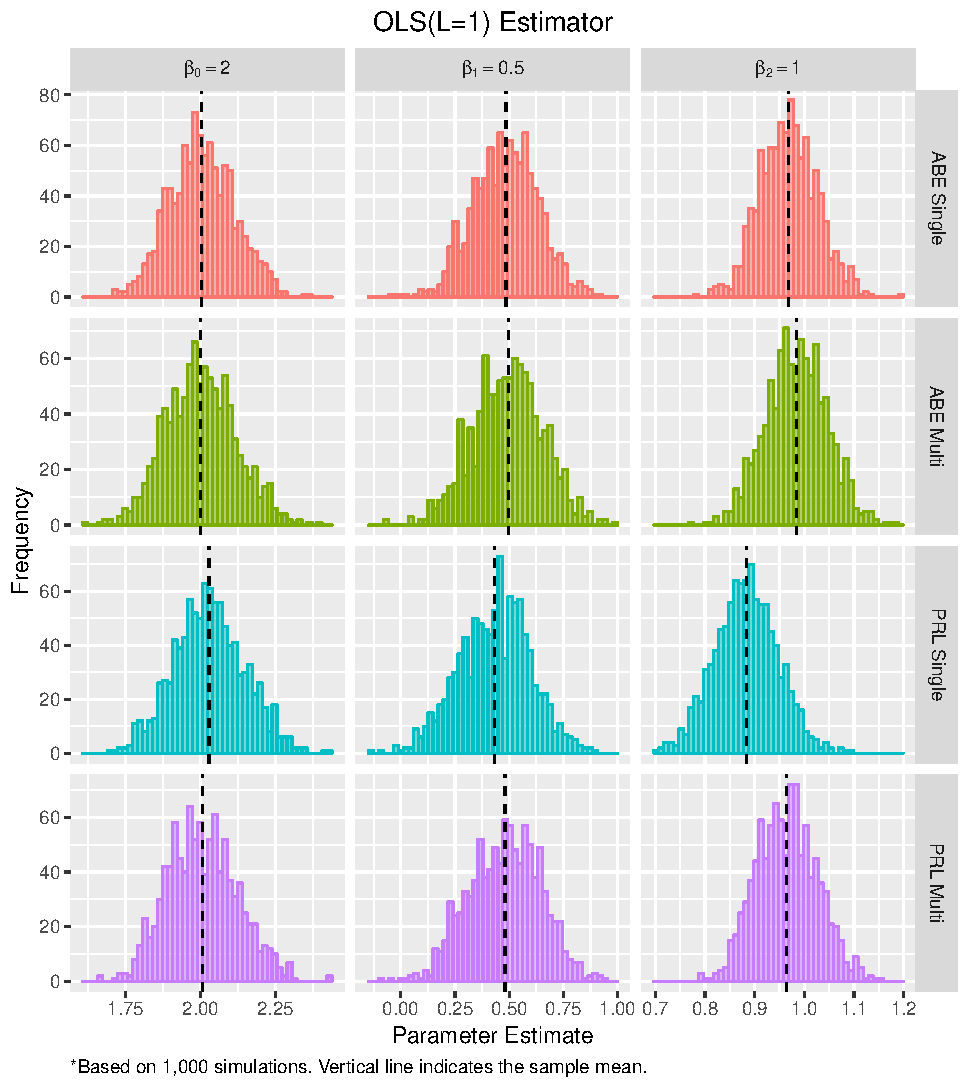
\includegraphics[width=\textwidth]{./Figures/OLS(L=1)_hist.pdf}
\label{ols}
\end{center}
\end{figure}


\newpage



\section{Appendix:  Implementation Notes}

\subsection{Proofs}
\subsection{Lemma 1}Consider,
\begin{equation}
\hat{\mu} = a_1X_{1} + a_2 X_2 -  a_3 \kappa \label{mu} \end{equation}
which has the following expectation,
$$ E[\hat{\mu}] = (a_1 \pi + a_2 (1-\pi))\mu + (a_1(1-\pi)+a_2\pi - a_3)\kappa $$
so that unbiased, requires
\begin{gather}
    a_1\pi + a_2(1-\pi) = 1 \implies a_2(a_1) = \frac{1}{1-\pi} - \frac{a_1 \pi}{1-\pi} \\
    a_1 (1-\pi) + a_2 \pi = a_3 \implies a_3(a_1) = \frac{\pi}{1-\pi}  + \frac{a_1 - 2a_1 \pi}{1-\pi} 
\end{gather}
Hence we can write $\hat{\mu}$ as a function of $a_1$,  
 $$\hat{\mu}(a_1) = a_1 X_1 +  \left(\frac{1}{1-\pi} - \frac{a_1 \pi}{1-\pi}\right)  X_2 - \left(\frac{\pi}{1-\pi} + \frac{a_1 - 2a_1\pi}{1-\pi}\right)\kappa $$ 
When $a_1 = \frac{1}{\pi}$, then $\hat{\mu} = \hat{\mu}_1$; and if $a_1 = 0$ then $\hat{\mu}=\hat{\mu_2}$. 

We can write:
\begin{align*}
\hat{\mu} &= (a_1 \pi) \hat{\mu}_1 + (1-a_1\pi) \hat{\mu}_2 + a_1(1-\pi)\kappa  + \frac{\pi}{1-\pi}(1-a_1)\kappa - \left(\frac{\pi}{1-\pi} + \frac{a_1 - 2a_1\pi}{1-\pi}\right)\kappa  \\
&=  (a_1 \pi) \hat{\mu}_1 + (1-a_1\pi) \hat{\mu}_2 - (a_1\pi)\kappa
\end{align*}

Hence any unbiased estimator $\hat{\mu}$ that uses $X_1$ and $X_2$ can be written as a linear combination of estimators using only $X_1$ or $X_2$.  

\subsection{Variance formulas}
\Var{X_1}$ and $\Var{X_2}$ are calculated using the law of total variance, using the random variable $D = 1$ if $X_1$ is drawn from the correct distribution (and $X_2$ is drawn from the incorrect distribution), and $D=0$ otherwise:
\begin{align*} \Var{X_1} &= E[\Var{X_1 | D}] + \Var{E[X_1| D]} \\ 
&= P(D=1)\sigma^2 +  P(D=0)\omega^2 + \Var{\mu D + \kappa (1-D)} \\
&= \pi \sigma^2 + (1-\pi) \omega^2 + \pi(1-\pi)(\mu-\kappa)^2
\end{align*}
The same trick can be applied to calculate $\Var{X_2}$


\subsection{implementation notes}

Let's talk about what I need to include here.  Here are some ideas:

Formulas for SE of SW estimator.

Details about implementation of fastLink algorithm. Also
\begin{itemize}
\item what threshold level I use for the fastLink algorithm (0.6)
\item what nonparametric technique I use for AHL (nearest neighbor) 
\item how I choose z in LL when there are multiple matches (randomly)
\item how I calculate standard errors for all of the estimators (using formulas for now)
\item how I standardize the variables for matching (nysiis function in R)
\item I change Step 2 in the ABE algorithm to restrict the all observations with unique first name, last name, date of birth, and $(x_1, x_2)$ combinations. 
\item  When allowing for multiple matches, I count as matches all record pairs with the same name, and the difference in recorded birth years is within two (or five) years.  That is, I designate all potential matches that arise in Step 3 as matches. 
\end{itemize}



\section{More MSE Tables}

\begin{table}

\caption{\label{tab:}MSE ratio for $\hat{\mu}^*$ and $\hat{\mu}^{AHL}$ for $N=1,000$ and $(\mu, \sigma^2, \kappa, \omega^2) = ($0,1,1,1)}
\centering
\begin{tabular}[t]{ccccccccccc}
\toprule
\multicolumn{1}{c}{ } & \multicolumn{10}{c}{$\hat{\pi}}$} \\
\cmidrule(l{3pt}r{3pt}){2-11}
$\pi$ & 0.05 & 0.1 & 0.15 & 0.2 & 0.25 & 0.3 & 0.35 & 0.4 & 0.45 & 0.5\\
\midrule
0.1 & 0.585 & 1.542 & 0.661 & 0.301 & 0.197 & 0.166 & 0.177 & 0.245 & 0.482 & 1\\
0.2 & 0.094 & 0.220 & 0.652 & 1.273 & 0.761 & 0.460 & 0.380 & 0.424 & 0.647 & 1\\
0.3 & 0.035 & 0.062 & 0.125 & 0.299 & 0.755 & 1.113 & 0.886 & 0.758 & 0.839 & 1\\
0.4 & 0.018 & 0.028 & 0.048 & 0.091 & 0.195 & 0.458 & 0.884 & 1.027 & 0.985 & 1\\
0.5 & 0.011 & 0.016 & 0.025 & 0.042 & 0.079 & 0.166 & 0.379 & 0.757 & 0.985 & 1\\
0.6 & 0.007 & 0.010 & 0.015 & 0.024 & 0.042 & 0.080 & 0.177 & 0.424 & 0.839 & 1\\
0.7 & 0.005 & 0.007 & 0.010 & 0.015 & 0.026 & 0.047 & 0.098 & 0.245 & 0.647 & 1\\
0.8 & 0.004 & 0.005 & 0.007 & 0.011 & 0.017 & 0.030 & 0.062 & 0.154 & 0.482 & 1\\
0.9 & 0.003 & 0.004 & 0.006 & 0.008 & 0.012 & 0.021 & 0.042 & 0.104 & 0.360 & 1\\
\bottomrule
\end{tabular}
\end{table}

\begin{table}

\caption{\label{tab:}MSE ratio for $\hat{\mu}^*$ and $\hat{\mu}^{AHL}$ for $N=1,000$ and $(\mu, \sigma^2, \kappa, \omega^2) = ($0,1,1,2)}
\centering
\begin{tabular}[t]{ccccccccccc}
\toprule
\multicolumn{1}{c}{ } & \multicolumn{5}{c}{$\hat{\pi}}$} \\
\cmidrule(l{3pt}r{3pt}){2-6}
$\pi$ & 0.05 & 0.1 & 0.15 & 0.2 & 0.25 & 0.3 & 0.35 & 0.4 & 0.45 & 0.5\\
\midrule
0.1 & 0.794 & 2.085 & 0.790 & 0.314 & 0.184 & 0.142 & 0.141 & 0.188 & 0.394 & 1\\
0.2 & 0.126 & 0.269 & 0.753 & 1.545 & 0.807 & 0.425 & 0.322 & 0.349 & 0.565 & 1\\
0.3 & 0.047 & 0.075 & 0.138 & 0.303 & 0.774 & 1.225 & 0.890 & 0.706 & 0.793 & 1\\
0.4 & 0.024 & 0.034 & 0.052 & 0.090 & 0.178 & 0.409 & 0.862 & 1.054 & 0.987 & 1\\
0.5 & 0.015 & 0.019 & 0.027 & 0.041 & 0.070 & 0.138 & 0.311 & 0.682 & 0.975 & 1\\
0.6 & 0.010 & 0.012 & 0.017 & 0.024 & 0.037 & 0.066 & 0.137 & 0.337 & 0.769 & 1\\
0.7 & 0.007 & 0.009 & 0.011 & 0.015 & 0.023 & 0.038 & 0.075 & 0.183 & 0.545 & 1\\
0.8 & 0.005 & 0.006 & 0.008 & 0.011 & 0.015 & 0.025 & 0.047 & 0.112 & 0.380 & 1\\
0.9 & 0.004 & 0.005 & 0.006 & 0.008 & 0.011 & 0.017 & 0.032 & 0.075 & 0.271 & 1\\
\bottomrule
\end{tabular}
\end{table}

\begin{table}

\caption{\label{tab:}MSE ratio for $\hat{\mu}^*$ and $\hat{\mu}^{AHL}$ for $N=1,000$ and $(\mu, \sigma^2, \kappa, \omega^2) = ($0,4,1,2)}
\centering
\begin{tabular}[t]{ccccccccccc}
\toprule
\multicolumn{1}{c}{ } & \multicolumn{10}{c}{$\hat{\pi}}$} \\
\cmidrule(l{3pt}r{3pt}){2-11}
$\pi$ & 0.05 & 0.1 & 0.15 & 0.2 & 0.25 & 0.3 & 0.35 & 0.4 & 0.45 & 0.5\\
\midrule
0.1 & 0.938 & 1.288 & 0.932 & 0.622 & 0.478 & 0.431 & 0.452 & 0.555 & 0.776 & 1\\
0.2 & 0.258 & 0.522 & 0.959 & 1.150 & 0.953 & 0.770 & 0.701 & 0.736 & 0.869 & 1\\
0.3 & 0.105 & 0.185 & 0.348 & 0.646 & 0.980 & 1.063 & 0.976 & 0.921 & 0.947 & 1\\
0.4 & 0.056 & 0.089 & 0.152 & 0.275 & 0.499 & 0.802 & 0.997 & 1.015 & 0.995 & 1\\
0.5 & 0.034 & 0.052 & 0.083 & 0.140 & 0.250 & 0.451 & 0.733 & 0.947 & 1.002 & 1\\
0.6 & 0.023 & 0.034 & 0.051 & 0.083 & 0.143 & 0.259 & 0.475 & 0.769 & 0.967 & 1\\
0.7 & 0.017 & 0.023 & 0.035 & 0.054 & 0.091 & 0.162 & 0.310 & 0.583 & 0.899 & 1\\
0.8 & 0.012 & 0.017 & 0.025 & 0.038 & 0.062 & 0.110 & 0.211 & 0.434 & 0.809 & 1\\
0.9 & 0.010 & 0.013 & 0.019 & 0.028 & 0.045 & 0.078 & 0.151 & 0.327 & 0.714 & 1\\
\bottomrule
\end{tabular}
\end{table}

\begin{table}

\caption{\label{tab:}MSE ratio for $\hat{\mu}^*$ and $\hat{\mu}^{AHL}$ for $N=1,000$ and $(\mu, \sigma^2, \kappa, \omega^2) = ($0,1,4,2)}
\centering
\begin{tabular}[t]{cccccc}
\toprule
\multicolumn{1}{c}{ } & \multicolumn{5}{c}{$\hat{\pi}}$} \\
\cmidrule(l{3pt}r{3pt}){2-6}
$\pi$ & 0.1 & 0.2 & 0.3 & 0.4 & 0.5\\
\midrule
0.1 & 1.399 & 0.160 & 0.121 & 0.221 & 1\\
0.2 & 0.062 & 1.146 & 0.361 & 0.391 & 1\\
0.3 & 0.016 & 0.157 & 1.052 & 0.726 & 1\\
0.4 & 0.007 & 0.044 & 0.356 & 1.012 & 1\\
0.5 & 0.004 & 0.020 & 0.120 & 0.719 & 1\\
0.6 & 0.003 & 0.011 & 0.057 & 0.387 & 1\\
0.7 & 0.002 & 0.007 & 0.033 & 0.219 & 1\\
0.8 & 0.001 & 0.005 & 0.021 & 0.136 & 1\\
0.9 & 0.001 & 0.004 & 0.015 & 0.092 & 1\\
\bottomrule
\end{tabular}
\end{table}

\begin{table}

\caption{\label{tab:}MSE ratio for $\hat{\mu}^*$ and $\hat{\mu}^{AHL}$ for $N=1,000$ and $(\mu, \sigma^2, \kappa, \omega^2) = ($0,1,1,10)}
\centering
\begin{tabular}[t]{ccccccccccc}
\toprule
\multicolumn{1}{c}{ } & \multicolumn{10}{c}{$\hat{\pi}}$} \\
\cmidrule(l{3pt}r{3pt}){2-11}
$\pi$ & 0.05 & 0.1 & 0.15 & 0.2 & 0.25 & 0.3 & 0.35 & 0.4 & 0.45 & 0.5\\
\midrule
0.1 & 2.247 & 4.501 & 1.933 & 0.739 & 0.386 & 0.263 & 0.230 & 0.274 & 0.508 & 1\\
0.2 & 0.400 & 0.730 & 1.574 & 2.456 & 1.414 & 0.729 & 0.503 & 0.488 & 0.694 & 1\\
0.3 & 0.153 & 0.218 & 0.344 & 0.623 & 1.192 & 1.546 & 1.150 & 0.883 & 0.902 & 1\\
0.4 & 0.080 & 0.101 & 0.136 & 0.202 & 0.335 & 0.612 & 1.010 & 1.125 & 1.033 & 1\\
0.5 & 0.049 & 0.058 & 0.072 & 0.096 & 0.140 & 0.231 & 0.425 & 0.757 & 0.980 & 1\\
0.6 & 0.033 & 0.037 & 0.044 & 0.055 & 0.075 & 0.114 & 0.202 & 0.412 & 0.790 & 1\\
0.7 & 0.024 & 0.026 & 0.030 & 0.036 & 0.047 & 0.067 & 0.114 & 0.237 & 0.587 & 1\\
0.8 & 0.018 & 0.019 & 0.021 & 0.025 & 0.032 & 0.044 & 0.072 & 0.150 & 0.428 & 1\\
0.9 & 0.014 & 0.015 & 0.016 & 0.019 & 0.023 & 0.031 & 0.050 & 0.102 & 0.317 & 1\\
\bottomrule
\end{tabular}
\end{table}







\newpage
\singlespacing
\bibliography{./Deadlines/proposal_bib} 
\bibliographystyle{aer}

\end{document}